
\clearpage
\section{Le classement des documents}
\label{bkm:Ref434830029}\label{bkm:Ref434828324}

\begin{wrapfigure}[14]{l}{6.5cm}   % [x] Wie manche Zeile soll sich um die Grafik "brechen"
  \vspace{-35pt}      % Grundwert war 20; mit 30 schön oben beim Text ausgerichtet
  \begin{center}
    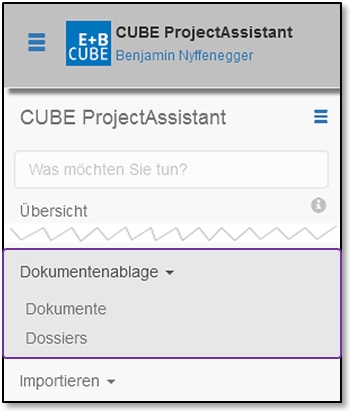
\includegraphics[width=1\linewidth]{../chapters/11_Dokumentenablage/pictures/11_Menu_Dokumentenablage.jpg}
  \end{center}
  \vspace{-20pt}
  \caption{Utilisation du classement des documents}
  \vspace{-10pt}
\end{wrapfigure}

Choisissez l'élément 'Classement des documents' dans le menu à gauche. Les sous-éléments 'Documents' et 'Dossiers' apparaissent.

\vspace{\baselineskip}

Le fonction de classement des documents est utilisée pour gérer et modifier les documents. Quand des documents ou leurs métadonnées sont modifiés, ils reçoivent un nouveau numéro de version dans CUBE PA. Les fonction d'extraction et de réintroduction de documents assurent qu'un document ne peut être modifié que par un seul utilisateur à la fois. D'autre part, l'attribution de versions aux documents assure que tous les participants au projet peuvent faire référence à des versions de documents uniques. 

\vspace{1cm}  

Les documents saisis ou chargés peuvent être classés dans des dossiers, qui peuvent ensuite être facilement téléchargés. Pour cette raison, la création et la gestion de dossiers sont décrites en premier dans ce chapitre.

\vspace{\baselineskip}

La gestion de documents est ensuite expliquée dans les détails.

\subsection{Dossiers}
\label{bkm:Ref442544219}\subsubsection{Créer des dossiers}

Un dossier est un ensemble de documents associés. Un exemple classique est un dossier d'approbation des plans ou un avant-projet. Les dossiers permettent de grouper plusieurs documents chargés, dans le but qu'ils puissent ensuite être téléchargés ensemble en tant qu'archive ZIP. 

\begin{figure}[H]
\center{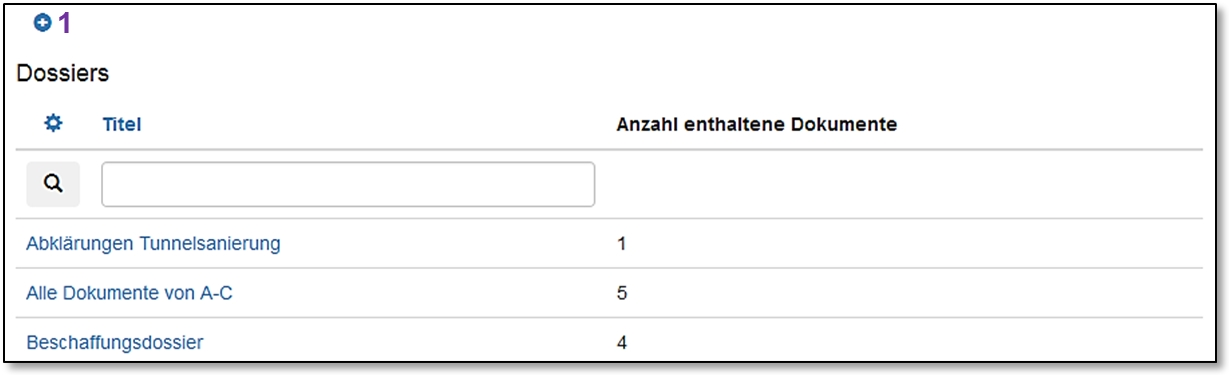
\includegraphics[width=1\linewidth]{../chapters/11_Dokumentenablage/pictures/11-1-1_UebersichtDossiers.jpg}}
\caption{Créer un nouveau dossier}
% \label{fig:speciation}
\end{figure}

Pour créer un nouveau dossier, sélectionnez l'élément de menu 'Classement des documents' et ensuite le sous-élément 'Dossiers'. Cliquez ensuite sur le symbole plus (ajouter) 
\includegraphics[height=12pt]{/Icons/Plussymbol.jpg} \col{(1)}.

\vspace{\baselineskip}

Le masque de saisie pour un dossier est apparaît :

\begin{figure}[H]
\center{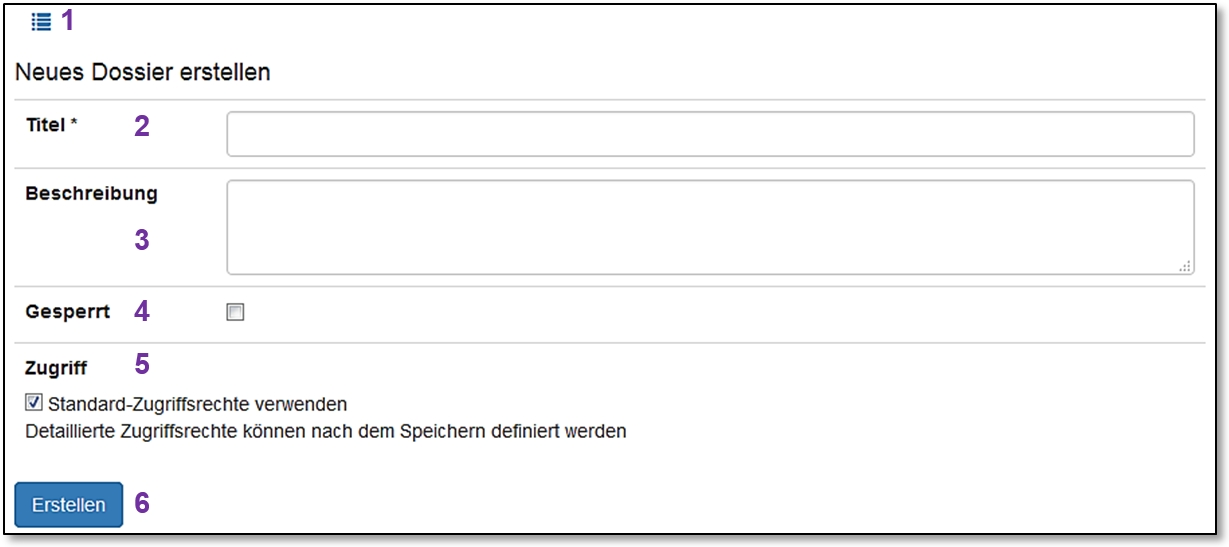
\includegraphics[width=1\linewidth]{../chapters/11_Dokumentenablage/pictures/11-1-1_DossierEingabemaske.jpg}}
\caption{Masque de saisie pour un nouveau dossier}
% \label{fig:speciation}
\end{figure}

Saisissez un titre significatif \col{(2)} pour le nouveau dossier. Comme plusieurs dossiers peuvent aborder le même sujet, il est recommandé d'indiquer la date dans le titre, comme par exemple 'Étude de faisabilité XY. Août 2015'. Il est également recommandé de vérifier, avant de créer un nouveau dossier, si un dossier avec un titre similaire existe déjà. Si tel est le cas, le même titre exactement devrait être utilisé, par exemple 'Étude de faisabilité XY. Août 2015' et 'Étude de faisabilité XY. Décembre 2015'. Une description détaillée \col{(3)} peut être ajoutée si nécessaire. Les dossiers peuvent être verrouillés contre les modifications. Si cette fonction est activée, l'ajout et le retrait des documents du dossier n'est pas possible. Pour ce faire, sélectionnez l'option 'Verrouillé' \col{(4)} en cochant la case correspondante. Le dossier ne sera plus disponible pour sélection dans le menu déroulant des documents. En cas de besoin, les dossiers peuvent être protégés par des droits d'accès. Si des droits d'accès spéciaux ne sont pas nécessaires, gardez la case 'Utiliser les droits d'accès par défaut' sous 'Accès' \col{(5)} cochée. Si le dossier ne doit être accessible qu'à certains groupes/utilisateurs, décochez la case. Vous pouvez définir plus tard quel(s) utilisateur(s) ou groupe(s) peuvent accéder au dossier. Pour plus d'informations sur les droits d'accès, voir chapitre \ref{bkm:Ref442273510}. \newline

Quand toutes les informations désirées ont été saisies, créez le dossier en cliquant sur le bouton 'Créer' \col{(6)}. Pour retourner à l'aperçu/liste de tous les documents, cliquez sur le symbole de liste 
\includegraphics[height=12pt]{/Icons/Listensymbol_zurueck.jpg} \col{(1)}.

\vspace{\baselineskip}

Quand un dossier est créé avec le bouton 'Créer', la vue d'ensemble suivante s'affiche :

\begin{figure}[H]
\center{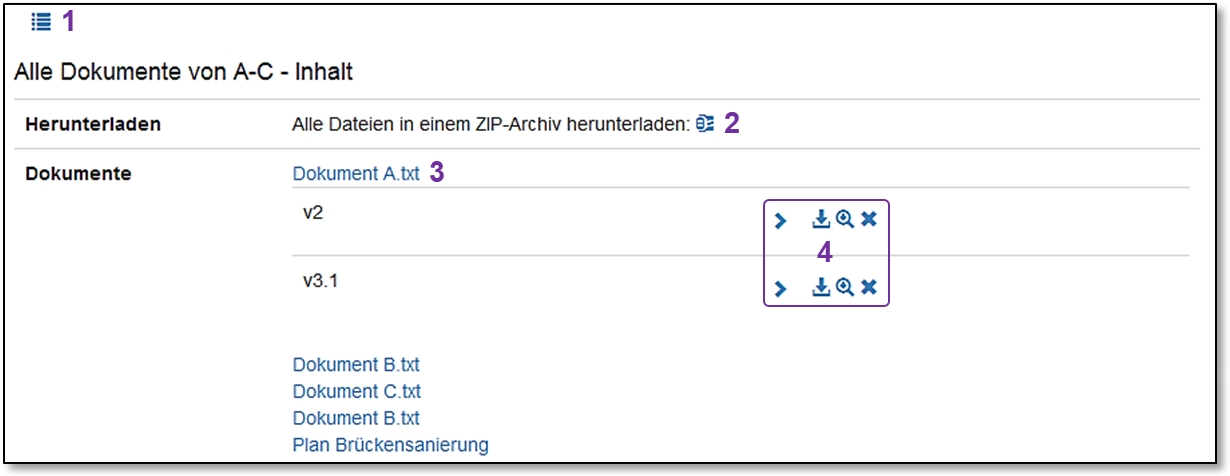
\includegraphics[width=1\linewidth]{../chapters/11_Dokumentenablage/pictures/11-1-1_UebersichtEinesDossiers.jpg}}
\caption{Vue d'ensemble du dossier}
% \label{fig:speciation}
\end{figure}

La saisie du dossier est maintenant visible. Cliquez sur le symbole ZIP 
\includegraphics[height=12pt]{/Icons/ZIPSymbol.jpg} \col{(2)} pour télécharger les documents contenus dans le dossier. Cliquez sur le titre d'un document en bleu \col{(3)} pour afficher les options (vous trouverez les explications relatives aux options plus bas). Les versions principales ou secondaires du document qui sont associées au dossier sont indiquées. Cliquez à nouveau sur le titre du document en bleu pour cacher les options.

Cliquez sur le symbole de liste 
\includegraphics[height=12pt]{/Icons/Listensymbol_zurueck.jpg} \col{(1)} pour retourner à l'aperçu/liste de tous les documents.

\vspace{\baselineskip}

Le classement des documents dans un dossier se fait dans la rubrique 'Documents' (Choisir l'élément 'Classement des documents' dans le menu à gauche puis le sous-élément 'Documents'). Pour ajouter des documents à un dossier, les documents doivent d'abord être chargés (voir chapitre \ref{bkm:Ref442769978}).

\subsubsection{Afficher et modifier un dossier}

Les options suivantes sont disponibles dans l'aperçu des dossiers :

\begin{figure}[H]
\center{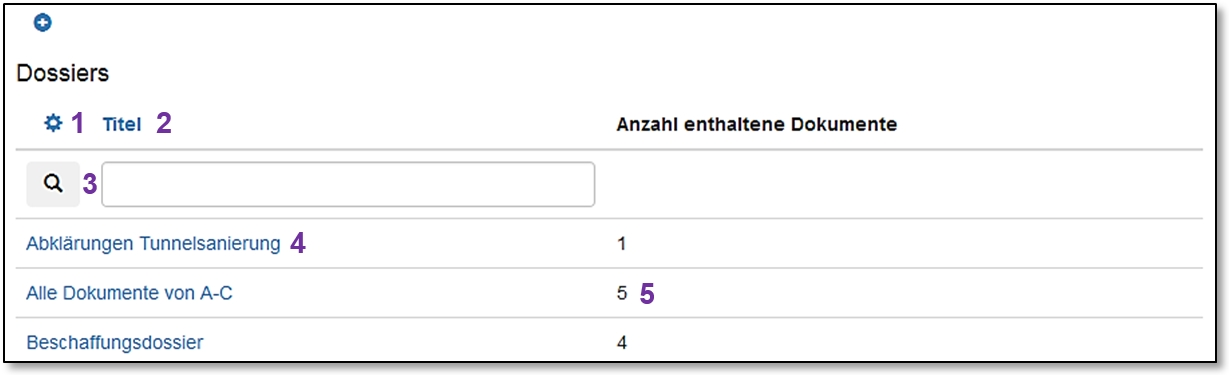
\includegraphics[width=1\linewidth]{../chapters/11_Dokumentenablage/pictures/11-1-2_UebersichtAllerDossiers.jpg}}
\caption{Aperçu de tous les dossiers}
% \label{fig:speciation}
\end{figure}

Vous pouvez afficher et masquer des colonnes en utilisant le symbole de configuration 
\includegraphics[height=12pt]{/Icons/SpaltenEinst.jpg} \col{(1)} (Ceci n'a pas d'effet dans l'aperçu des dossiers puisqu'il n'y a qu'une seule colonne). Cliquez sur 'Titre' \col{(2)} pour trier les dossiers par ordre alphabétique de A à Z. Cliquez à nouveau pour les trier par ordre alphabétique de Z à A.

\vspace{\baselineskip}

\textbf{Recherche :} Vous pouvez chercher un dossier dans l'aperçu. Sans utiliser un caractère de remplacement (*), vous pouvez directement saisir un mot clé et cliquer le symbole de loupe 
\includegraphics[height=12pt]{/Icons/Lupe_kl.jpg} \col{(3)} ou appuyer sur la touche Entrée. Tous les documents contenant le mot clé seront affichés. \newline

Cliquez sur le titre du dossier \col{(4)} pour aller directement à l'aperçu détaillé et au mode de modification du dossier. Dans l'aperçu détaillé vous pouvez également voir combien de documents contient le dossier \col{(5)}. La suppression de dossiers n'est pas possible pour le moment. \newline

Si vous ouvrez un dossier en cliquant sur son titre \col{(4)}, vous pouvez aussi voir tous les documents qu'il contient :

\begin{figure}[H]
\center{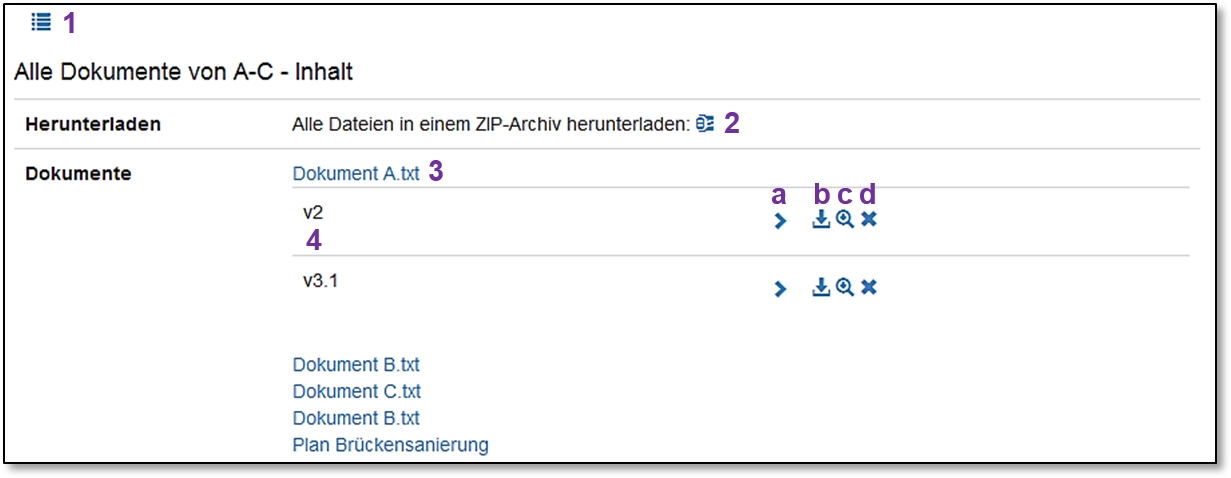
\includegraphics[width=1\linewidth]{../chapters/11_Dokumentenablage/pictures/11-1-2_DetailsEinesDossiers.jpg}}
\caption{Aperçu détaillé d'un dossier}
% \label{fig:speciation}
\end{figure}

Cliquez sur le symbole de liste 
\includegraphics[height=12pt]{/Icons/Listensymbol_zurueck.jpg} \col{(1)} pour retourner à l'aperçu de tous les dossiers. Vous pouvez télécharger tous les documents contenus dans le dossier en cliquant sur le symbole ZIP 
\includegraphics[height=12pt]{/Icons/ZIPSymbol.jpg} \col{(2)}. Une fenêtre de dialogue apparaît dans laquelle vous pouvez choisir si vous voulez sauvegarder l'archive ZIP sur votre ordinateur ou simplement l'ouvrir. La fenêtre dépend du navigateur que vous utilisez. \newline

Vous trouverez aussi une liste de tous les documents que contient le dossier. Cliquez sur le titre du document en bleu \col{(3)} pour afficher plus d'options. La version du document associée au dossier est indiquée \col{(4)}. \newline

Les options suivantes sont disponibles :
Avec le symbole de croix 
\includegraphics[height=12pt]{/Icons/blKreuzchen.jpg} \col{(d)} vous pouvez supprimer une version spécifique d'un document associé au dossier. Vous devez ensuite confirmer l'avertissement de sécurité.

\begin{figure}[H]
\center{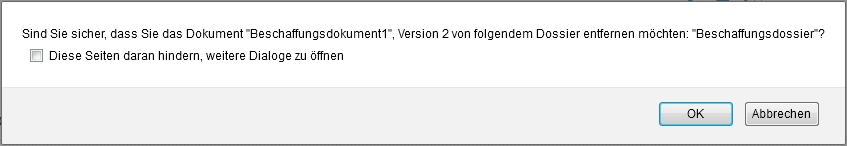
\includegraphics[width=.8\linewidth]{../chapters/11_Dokumentenablage/pictures/11-1-2_DokLoeschen_Meldung.jpg}}
% \caption{Detailansicht des Dossiers}
% \label{fig:speciation}
\end{figure}

Le symbole de loupe 
\includegraphics[height=12pt]{/Icons/Lupe.jpg} \col{(c)} vous dirige vers la saisie du document. Vous pouvez modifier la saisie du document, charger une nouvelle version du document, etc. Pour plus de détails sur le classement des documents, voir chapitre \ref{bkm:Ref442273482}. Le symbole de téléchargement 
\includegraphics[height=12pt]{/Icons/Download.jpg} \col{(b)} vous permet de télécharger une version spécifique du document (c'est-à-dire pas le dossier en entier). Selon le type de document, vous pouvez prévisualiser un document spécifique en ligne. Si cette option est disponible, une flèche orientée vers la droite 
\includegraphics[height=12pt]{/Icons/Pfeil_rechts.jpg} \col{(a)} est visible. Cliquez sur la flèche pour ouvrir la prévisualisation dans une petite fenêtre. Cliquez sur la flèche orientée maintenant vers le bas pour fermer la prévisualisation :

\begin{figure}[H]
\center{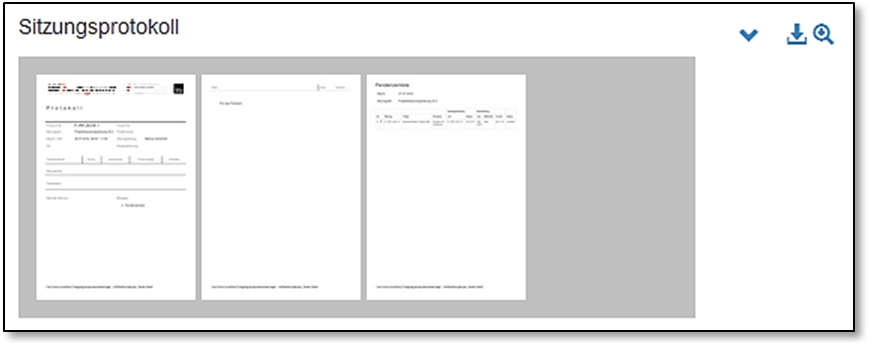
\includegraphics[width=0.75\linewidth]{../chapters/11_Dokumentenablage/pictures/11-1-2_Vorschau.jpg}}
\caption{Prévisualisation d'un document}
% \label{fig:speciation}
\end{figure}

\pagebreak

Cliquez sur une des pages de la prévisualisation pour ouvrir une visualisation détaillée de cette page :

\vspace{\baselineskip}

\begin{wrapfigure}[12]{r}{9cm}   % [x] Wie manche Zeile soll sich um die Grafik "brechen"
  \vspace{-30pt}      % Grundwert war 20; mit 30 schön oben beim Text ausgerichtet
  \begin{center}
    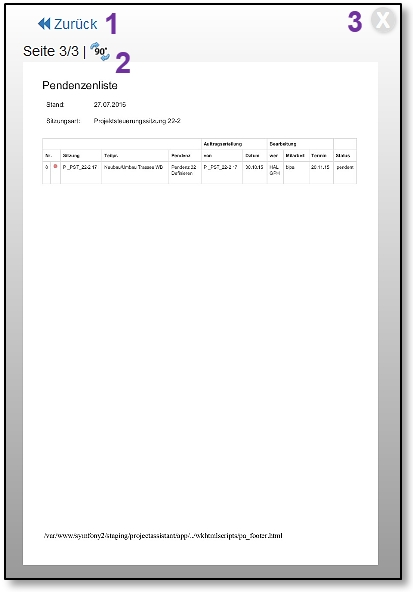
\includegraphics[height=110mm]{../chapters/11_Dokumentenablage/pictures/11-1-2_VorschauDetails.jpg}
  \end{center}
  \vspace{-20pt}
  \caption{Visualisation détaillée d'une page}
  \vspace{-10pt}
\end{wrapfigure}
En haut à gauche se trouve la navigation. Vous pouvez voir combien de pages contient le document et naviguer parmi les pages du document en cliquant les boutons 'Précédent' et 'Suivant' \col{(1)}. En cas de besoin (par exemple pour une carte ou un plan), vous pouvez tourner la page avec le symbole '90°' - cliquez une deuxième fois pour tourner la page de 90° supplémentaires, etc. Pour fermer la visualisation, cliquez sur le bouton 'X' \col{(3)}.

\vspace{5cm}

\subsubsection{Gérer les droits d'accès aux dossier}
\label{bkm:Ref442273510}
Pour chaque dossier, vous pouvez décider qui peut le lire, modifier, et/ou supprimer (la suppression de dossiers n'est pas disponible pour le moment). Vous pouvez attribuer les droits d'accès pour un ou plusieurs groupe(s) ou utilisateur(s). La procédure est décrite au chapitre \ref{bkm:Ref442869495} et est similaire à l'attribution de droits d'accès pour les documents.

\pagebreak
\subsection{Documents}
\label{bkm:Ref442273482}

\subsubsection{Aperçu des documents (Recherche de documents)}
\label{bkm:Ref443047823}

Choisissez l'élément 'Classement des documents' dans le menu à gauche puis le sous-élément 'Documents'. Une liste des documents saisis/chargés est affichée dans l'aperçu des documents.

\begin{figure}[H]
\center{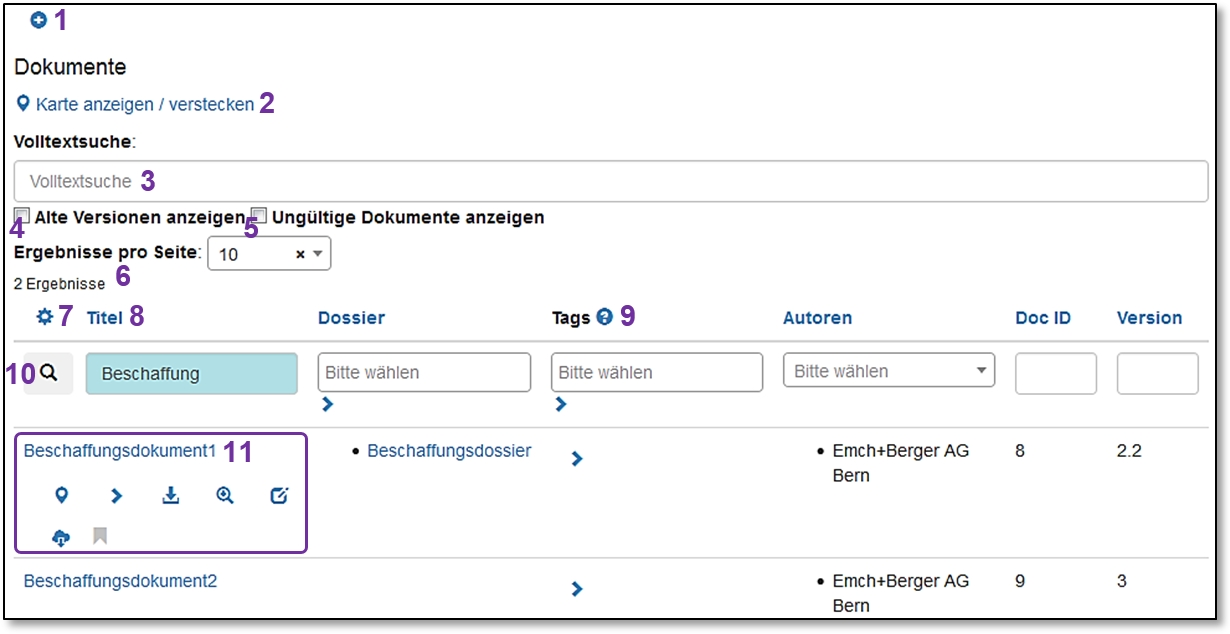
\includegraphics[width=1\linewidth]{../chapters/11_Dokumentenablage/pictures/11-2-1_DokumentenUebersicht.jpg}}
\caption{Aperçu des documents}
% \label{fig:speciation}
\end{figure}

Pour ajouter des nouveaux documents, cliquez sur le symbole plus (ajouter) 
\includegraphics[height=12pt]{/Icons/Plussymbol.jpg} \col{(1)}. Pour plus d'informations, voir chapitre \ref{bkm:Ref442770648}. Le symbole de filtre 
\includegraphics[height=12pt]{/Icons/Filter.jpg} \col{(2)} vous permet d'afficher ou de masquer les fonctions de filtre avancées (voir 'Filtre avancé' plus bas (\ref{bkm:Ref201704051})). Le symbole d'épingle \col{(3)} vous permet d'afficher ou de masquer une carte Google Maps. Sur la carte, tous les documents liés à la recherche et liés à Google Maps sont affichés. \newline

Des structures de tags (mots-clés) peuvent être mises en place sur mesure. Ces structures sont comparables aux structures de dossiers dans un explorateur de fichiers. Cliquez sur le titre d'une structure de tags \col{(4)} pour naviguer la structure et effectuer une recherche selon les tags. Pour plus d'informations, se référer au chapitre \ref{bkm:Ref201801849} (Tags hiérarchiques : Recherche de document dans une 'structure de dossiers'). \newline

La recherche plein texte \col{(5)} permet de chercher les saisies en fonction de mots-clé. Après avoir saisi un mot-clé, cliquez sur le symbole de loupe 
\includegraphics[height=12pt]{/Icons/Lupe_kl.jpg} \col{(6)} ou appuyez sur la touche Entrée. Plusieurs mots-clé peuvent être saisis. Si vous cherchez un groupe de mots spécifique, écrivez-le entre guillemets. Avec la recherche plein texte, les titres de documents et de dossiers, les tags (étiquettes), et si techniquement possible, le contenu des documents sont cherchés. Sous la recherche plein texte, le nombre de résultats est affiché \col{(7)}.\\
Le symbole de configuration 
\includegraphics[height=12pt]{/Icons/SpaltenEinst.jpg} \col{(8)} vous permet de masquer les colonnes non utilisées. Après avoir choisi les colonnes désirées, cliquez 'Actualiser' et l'aperçu des documents sera mis à jour. \newline

En plus de la recherche plein texte, vous pouvez effectuer des recherches par colonne \col{(9)}, ou bien choisir à l'aide des menus déroulants quels documents vous voulez afficher. Cliquez sur les en-têtes en bleu pour trier les documents par ordre alphabétique de A à Z. Cliquez à nouveau pour les trier par ordre alphabétique de Z à A. Les documents chargés peuvent être étiquetés par le moyen de tags. Pour plus d'informations sur les tags, voir chapitre \ref{bkm:Ref442275849}.\newline
Les cases à cocher 
\includegraphics[height=12pt]{/Icons/selectbox.jpg} \col{(10)} vous permettent de choisir des documents (un ou plusieurs) et d'appliquer des actions comme 'Télécharger', 'Envoyer comme pièce jointe', et 'Envoyer en format imprimé' à la sélection. Pour plus d'informations, voir chapitre \ref{bkm:Ref201705445} (Panier à documents).

Quand vous cliquez sur une saisie de données dans la liste \col{(11)} (dans la colonne Titre, texte en bleu), des options s'affichent. Les options sont expliquées plus bas.

\vspace{\baselineskip}

\textbf{Filtre avancé:}\\
\label{bkm:Ref201704051}

Le symbole de filtre 
\includegraphics[height=12pt]{/Icons/Filter.jpg} \col{(1)} vous permet d'afficher et de masquer les fonctions de filtre avancées:

\begin{figure}[H]
\center{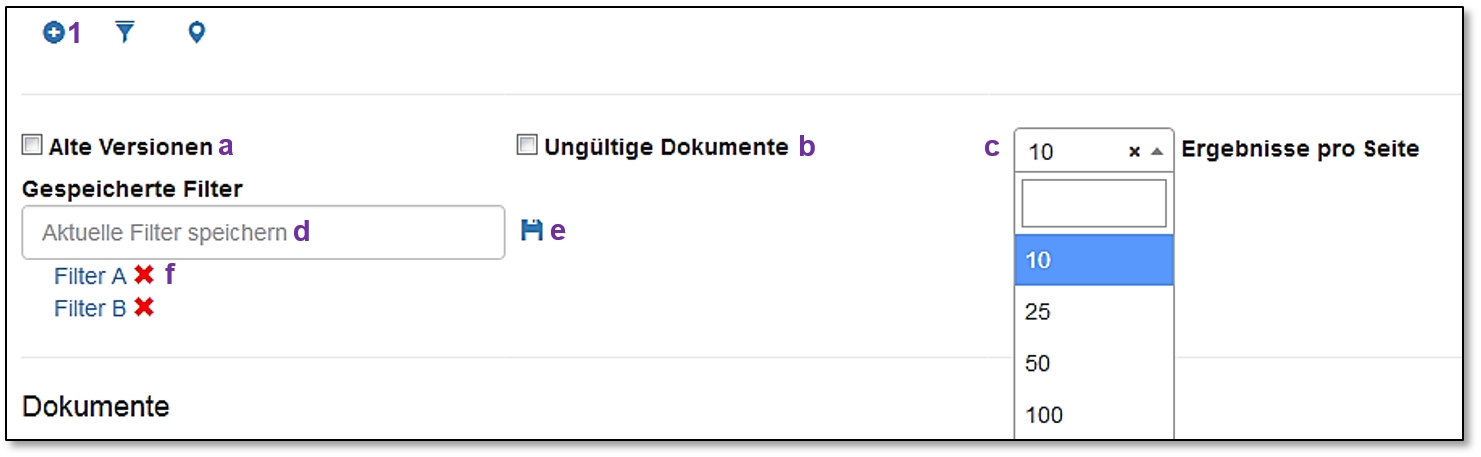
\includegraphics[width=.8\linewidth]{../chapters/11_Dokumentenablage/pictures/11-2-1_FilterEinstellen.jpg}}
\caption{Sauvegarder les paramètres de filtre}
% \label{fig:speciation}
\end{figure}

Pour inclure des anciennes versions et/ou des documents non valables dans la recherche, cochez la case 'Inclure anciennes versions' \col{(a)} et/ou la case 'Afficher les documents non valables' \col{(b)}. Sous 'Résultats par page' \col{(c)}, vous pouvez choisir le nombre de saisies à afficher par page.\\
Vous pouvez sauvegarder des paramètres de filtre pour usage ultérieur. Ceci tient compte de la recherche plein texte, des saisies de titres, de l'ID du document, ainsi que d'autres colonnes. Le nombre de résultats par page n'est pas sauvegardé dans les paramètres de filtre.\\
Une fois les paramètres de filtre désirés saisis, saisissez un titre pour le filtre \col{(d)} puis cliquez sur le symbole de sauvegarde 
\includegraphics[height=12pt]{/Icons/Diskette.jpg} \col{(e)}. Tous les paramètres de filtre sauvegardés sont affichés \col{(f)}. Un filtre sauvegardé peut être supprimé en cliquant sur la croix rouge 
\includegraphics[height=12pt]{/Icons/roKreuzchen.jpg} \col{(f)}.


\subsubsection{Ajouter un nouveau document}
\label{bkm:Ref442863508}\label{bkm:Ref442787515}\label{bkm:Ref442778397}\label{bkm:Ref442770648}\label{bkm:Ref442769978}

\begin{figure}[H]
\center{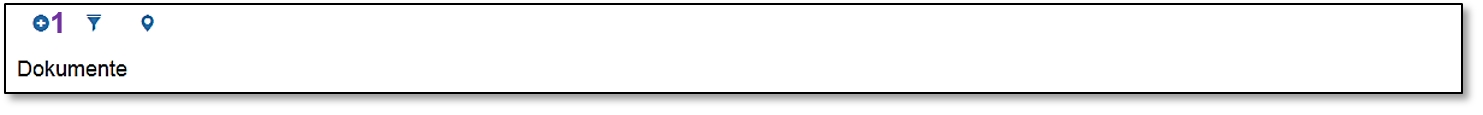
\includegraphics[width=1\linewidth]{../chapters/11_Dokumentenablage/pictures/11-2-2_DokumenteHochladen.jpg}}
% \caption{Neues Dokument hochladen}
% \label{fig:speciation}
\end{figure}

Cliquez sur le symbole plus (ajouter) 
\includegraphics[height=12pt]{/Icons/Plussymbol.jpg} \col{(1)}. Le masque de saisie pour un nouveau document s'affiche :

\begin{figure}[H]
\center{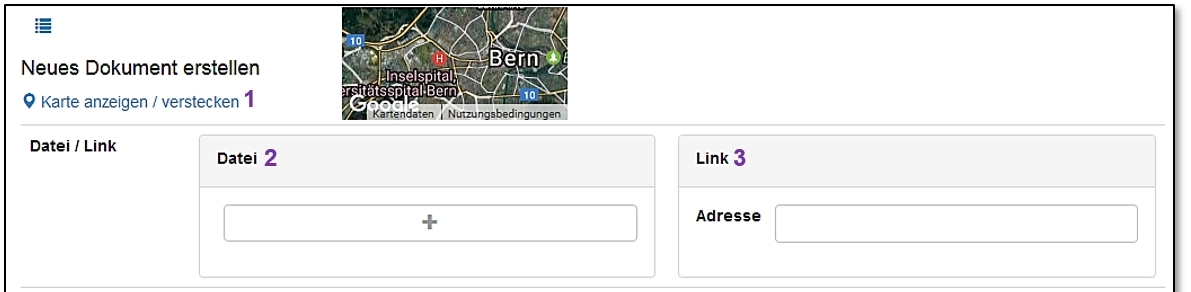
\includegraphics[width=1\linewidth]{../chapters/11_Dokumentenablage/pictures/11-2-2_NeuesDokuErstellen_A.jpg}}
\caption{Masque de saisie pour un nouveau document}
% \label{fig:speciation}
\end{figure}

Cliquez sur le lien 'Afficher / masquer carte' \col{(1)}, pour afficher Google Maps, ou pour passer à un affichage plus grand. Pour plus d'informations concernant l'association de documents à Google Maps, voir chapitre \ref{bkm:Ref442545553}. \newline

Vous pouvez maintenant choisir de charger un fichier \col{(2)} ou d'enregistrer un lien Internet \col{(3)}.

\vspace{\baselineskip}

\textbf{Charger un fichier:} \col{(2)}
\begin{figure}[H]
\center{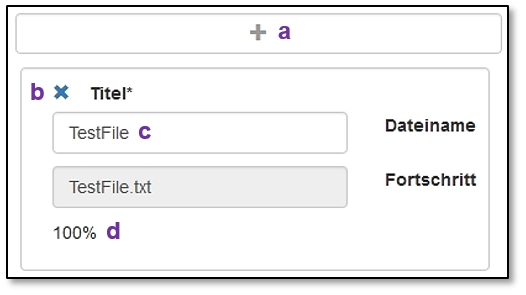
\includegraphics[width=.5\linewidth]{../chapters/11_Dokumentenablage/pictures/11-2-2_Dateititel.jpg}}
\caption{Charger un nouveau document}
\end{figure}

Cliquez sur le symbole plus gris 
\includegraphics[height=12pt]{/Icons/plus_grau.jpg} \col{(a)} et sélectionnez le fichier désiré. Alternativement, vous pouvez charger un ou plusieurs fichiers en glissant-déposant dans la 'zone plus'. Une fois un fichier sélectionné / déposé dans la 'zone plus', des champs additionnels sont affichés \col{(b-d)}. Si vous êtes en train de télécharger un grand fichier, vous pouvez voir le progrès de chargement du fichier \col{(d)} et s'il a été complètement chargé. Le titre est un champs de saisie obligatoire. Il est copié du nom du fichier \col{(c)} mais peut être modifié à tout moment. Si vous avez chargé le mauvais fichier, cliquez sur la petite croix 
\includegraphics[height=12pt]{/Icons/Kreuzchen.jpg} \col{(b)} pour enlever le fichier / la saisie. \\
Vous pouvez charger des fichiers supplémentaires. Pour ce faire, répétez ces étapes. 

\vspace{\baselineskip}

\textbf{Enregistrer un lien:} \col{(3)}
\begin{figure}[H]
\center{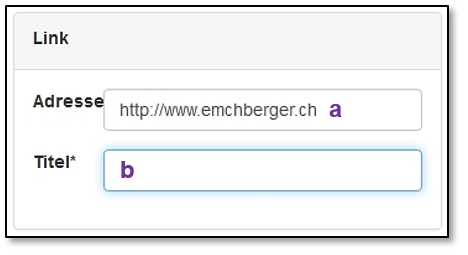
\includegraphics[width=.5\linewidth]{../chapters/11_Dokumentenablage/pictures/11-2-2_Linktitel.jpg}}
\caption{Enregistrer un lien}
\end{figure}

Sous 'Adresse' \col{(a)}, saisissez l'adresse web désiré. Un champs de saisie additionnel, 'Titre', apparaît \col{(b)} (champs obligatoire), dans lequel vous devez saisir un titre pour le lien.\\

Si vous avez saisi une adresse web non valable, le message suivant apparaît :

\begin{figure}[H]
\center{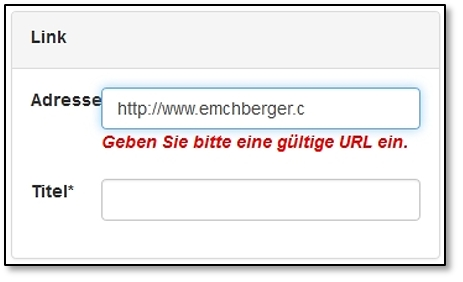
\includegraphics[width=.5\linewidth]{../chapters/11_Dokumentenablage/pictures/11-2-2_Link_Fehler.jpg}}
\caption{Enregistrer un lien}
\end{figure}

\vspace{\baselineskip}

Lorsque vous aurez chargé un fichier ou saisi une adresse web, vous pouvez remplir les champs de saisie suivants :

\begin{figure}[H]
\center{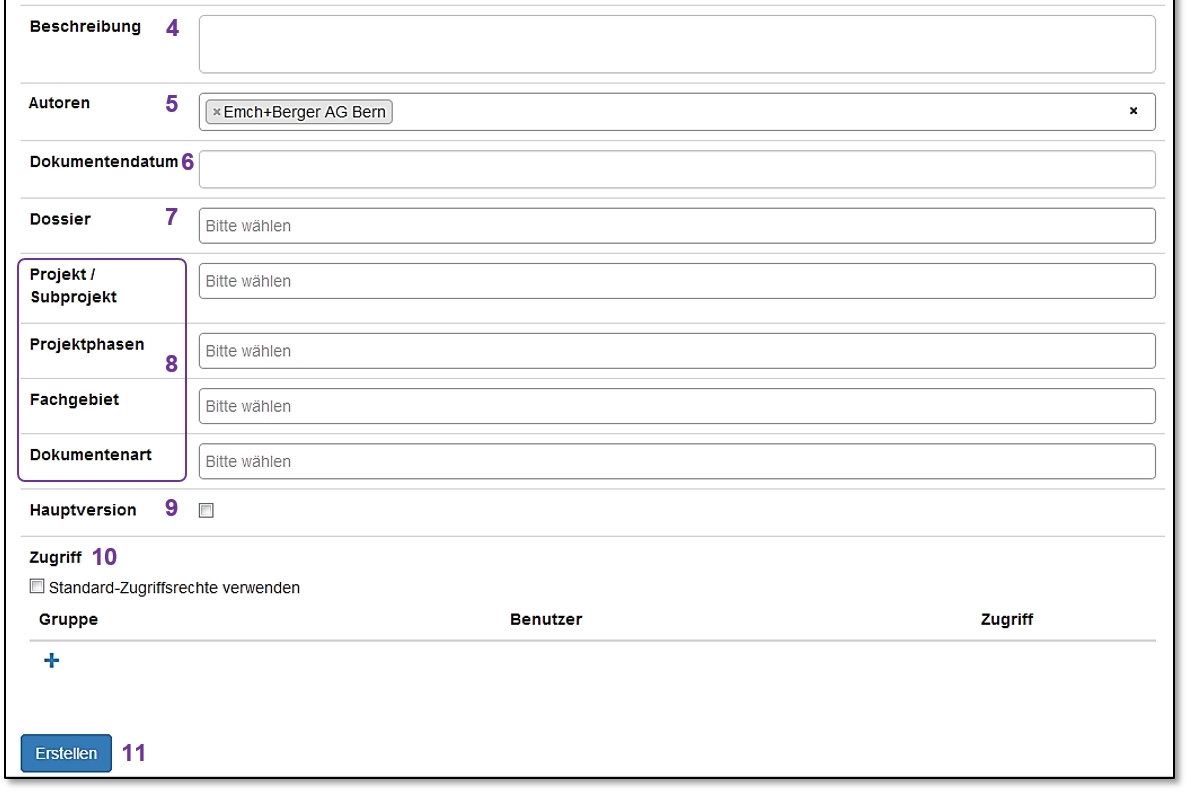
\includegraphics[width=1\linewidth]{../chapters/11_Dokumentenablage/pictures/11-2-2_NeuesDokuErstellen_B.jpg}}
\caption{Masque de saisie pour un nouveau document}
% \label{fig:speciation}
\end{figure}

%\vspace{\baselineskip}

Dans la description \col{(4)}, des notes supplémentaires peuvent être saisies. Sous 'Auteurs' \col{(5)}, vous pouvez choisir le(s) auteur(s) par l'intermédiaire d'un menu déroulant. L'auteur doit être saisi au préalable. Si un auteur n'est pas sur la liste, il peut être ajouté par l'administrateur. Vous avez la possibilité d'ajouter une date de document \col{(6)}. Pour classer un document dans un dossier (voir chapitre \ref{bkm:Ref442544219}), choisissez le dossier correspondant dans le menu déroulant \col{(7)} (le dossier doit déjà exister). Un document peut être classé dans plusieurs dossiers. Cliquez à nouveau sur le menu déroulant pour choisir plus de dossiers pour le document.

Des 'tags' (étiquettes) \col{(8)} peuvent être attribués à un document. Ceci permet d'effectuer des recherches de tags spécifiques pour trouver des documents de projets, phases de projet, domaines d'expertise, ou types de documents spécifiques. Les thèmes de tags (par exemple domaine d'expertise) et les tags individuels (par exemple passages à niveau, éclairage, exploitation, etc.) ne peuvent être définis ou ajoutés que par l'administrateur. Si un tag manque, veuillez contacter l'administrateur. La gestion détaillée des tags est décrite au chapitre \ref{bkm:Ref201801219} (Utilisation de tags). \newline

Si vous avez chargé plusieurs fichiers à la fois, une saisie séparée, mais avec les mêmes données (description, auteurs, dossiers, etc.) est créée pour chacun des fichiers. Ceci permet d'économiser du temps, surtout pour la création d'un dossier avec plusieurs documents ayant la même description, auteurs, etc. \newline

%Si un document n'est plus valable, il peut être exclu des résultats de recherche en cochant la case 'Non valable' \col{(8)}. Cette fonction n'est pas à confondre avec les versions de documents, qui font que les anciennes versions d'un document ne soient par défaut pas affichées dans les résultats de recherche.\newline

Vous pouvez indiquer si un fichier chargé constitue une version principale (V1, V2, V3, etc.) ou une version secondaire (V3.1, V3.2, etc.) d'un document. Si le fichier chargé est une version principale, cochez la case 'Version principale' \col{(9)}. Vous pouvez attribuer les droits d'accès par défaut \col{(10)} à un document ou autoriser l'accès à certaines personnes seulement. Les droits d'accès peuvent être adaptés et élargis à tout moment dans le mode de modification. Le chapitre \ref{bkm:Ref442869495} offre plus d'informations sur la gestion des droits d'accès. Pour créer un document, au moins un utilisateur doit avoir les droits d'accès au documents (en général l'utilisateur qui a créé le document).

Une fois toutes les informations nécessaires saisies, le document est chargé en cliquant le bouton 'Créer' \col{(11)} et les saisies sont enregistrées. \newline

\textbf{Remarque :} Un document peut être uniquement remplacé par un seul autre document. Si vous essayez de déposer plusieurs fichiers dans la fenêtre de chargement, le message d'erreur suivant s'affiche :

\begin{figure}[H]
\center{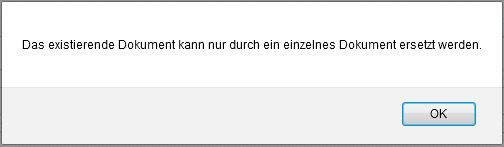
\includegraphics[width=0.75\linewidth]{1122_FehlerDokumentErsetzen.jpg}}
\caption{Message d'erreur pour le chargement de plusieurs fichiers}
% \label{fig:speciation}
\end{figure}

\textbf{Note :} Si uniquement les métadonnées d'un document sont modifiées et enregistrées, une nouvelle version du document ne sera pas créée. Les changements dans les métadonnées apparaîtront par contre dans l'historique du document. Similairement, si le même fichier est chargé (dans lequel aucun changement n'a été effectué) ou bien si un document a été extrait puis réintroduit sans aucune modification, CUBE PA ne crée pas une nouvelle version du document. Le message suivant s'affiche :

\begin{figure}[H]
\center{
\includegraphics[width=0.5\linewidth]{../chapters/11_Dokumentenablage/pictures/11-2-2_Meldung_gleicheDatei.jpg}}
\caption{Message : Nouvelle version de document non créée}
% \label{fig:speciation}
\end{figure}

Pour pouvoir continuer à travailler, vous devez d'abord cliquer sur 'OK' dans le dialogue ci-dessus.

\subsubsection{Documents avec lien Google Maps}
\label{bkm:Ref442545553}
Les documents peuvent être associés à Google Maps. De cette manière, les documents liés à un lieu spécifique peuvent être repérés, modifiés ou téléchargés. \\
Passez au mode de modification du document désiré avec le symbole de modification 
\includegraphics[height=12pt]{/Icons/Bearbeiten.jpg} (Dans le mode d'affichage, les liens Google Maps peuvent être visualisés mais vous ne pouvez pas créer, ajouter ou supprimer un lien).

% \vspace{\baselineskip}
\vspace{2mm}

\begin{wrapfigure}[15]{l}{6.5cm}
\vspace{-15pt}
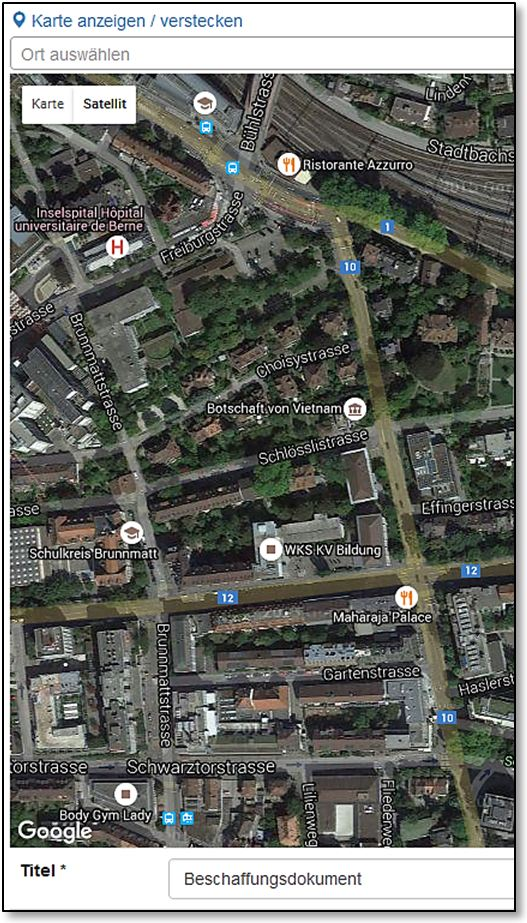
\includegraphics[height=110mm]{1123_GoogleMap.jpg}
% \caption{Status ändern}
\end{wrapfigure}

Pour lier un document à un lieu sur la carte, double-cliquez sur l'objet/le lieu désiré sur la carte. Vous pouvez également choisir un lieu prédéfini. Pour ce faire, cliquez sur le champ de saisie 'Choisir lieu' au-dessus de la carte et choisissez le lieu désiré.

\vspace{4mm}

\hspace{15mm} 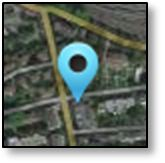
\includegraphics[height=20mm]{1123_GoogleMapNadel.jpg}

Le repère ci-dessus s'affiche. Vous pouvez ensuite déplacer ce repère vers un autre lieu par 'drag \& drop' (glisser-déposer).

\hspace{15mm} 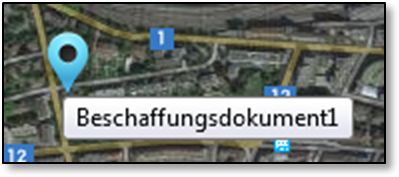
\includegraphics[height=20mm]{1123_GoogleMapText.jpg}

Déplacez le curseur au-dessus du repère pour voir quel ou quels documents sont liés à ce lieu. \\

Répétez les étapes ci-dessus pour ajouter plus de liens Google Maps. Pour supprimer un lien spécifique, cliquez sur le repère avec le bouton droit de la souris. Le dialogue suivant s'affiche, et vous demande de confirmer la suppression des coordonnées : 

\begin{figure}[H]
\center{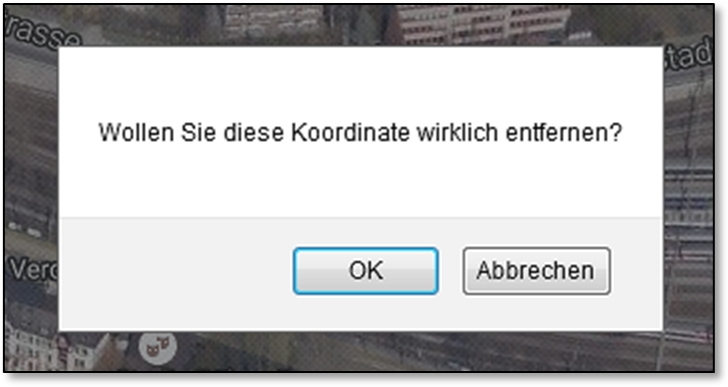
\includegraphics[width=0.5\linewidth]{../chapters/11_Dokumentenablage/pictures/11-2-3_DialogLoeschen.jpg}}
\caption{Supprimer un lien}
% \label{fig:speciation}
\end{figure}

\vspace{\baselineskip}
%\pagebreak

\textbf{Utiliser Google Maps dans CUBE PA :}

L'utilisation de Google Maps dans CUBE PA est identique à l'utilisation de Google Maps dans un navigateur. Cliquez et maintenez appuyé le bouton de la souris pour déplacer la carte. Si votre souris dispose d'une molette de défilement, utilisez cette dernière pour zoomer sur la carte. (Les touches de fonction comme Shift, Ctrl et Alt ne fonctionnent pas dans l'utilisation de la carte).

\vspace{\baselineskip}

\textbf{Rechercher un lieu :} 

\begin{figure}[H]
\center{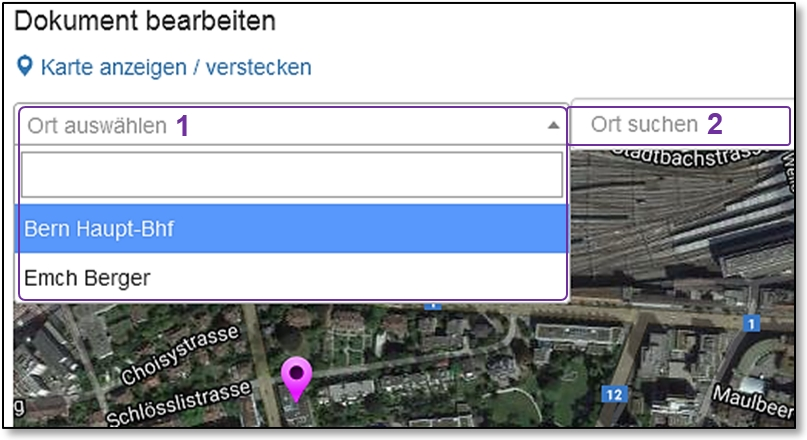
\includegraphics[width=0.6\linewidth]{../chapters/11_Dokumentenablage/pictures/11-2-3_GeographischSuchen.jpg}}
\caption{Rechercher un lien}
% \label{fig:speciation}
\end{figure}

Quand Google Maps est affiché dans l'aperçu des documents (cliquez sur 'Afficher / masquer la carte'), tous les documents avec un lien Google Maps sont affichés. Vous pouvez choisir un lieu du menu déroulant \col{(1)} ou chercher un lieu en saisissant l'information dans le champ \col{(2)} et en appuyant la touche Entrée. Google Maps naviguera au lieu désiré et affichera tous les documents qui y sont associés. Si vous avez filtré la liste de documents dans l'aperçu des documents, seuls les documents filtrés apparaîtront sur la carte. %\newline

\pagebreak
\textbf{Filtrer les documents selon la zone géographique :} \\

\begin{wrapfigure}[7]{r}{7cm}
  \vspace{-35pt}
  \begin{center}
    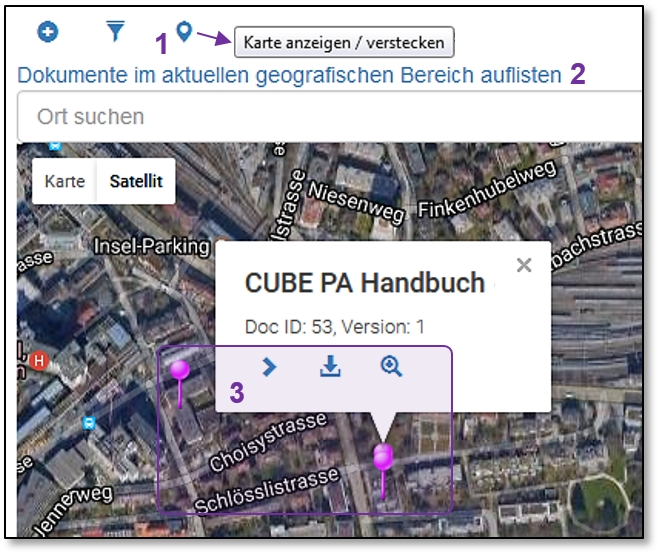
\includegraphics[height=55mm]{../chapters/11_Dokumentenablage/pictures/11-2-3_GeoBereichFilter.jpg}
  \end{center}
  \vspace{-20pt}
  % \caption{Geografische Bereiche filtern}
  \vspace{-10pt}
\end{wrapfigure}
Vous avez la possibilité de filtrer les documents qui sont dans la même zone géographique ou qui ont des coordonnées proches. Pour ce faire, cliquez sur 'Afficher / masquer carte' \col{(1)} pour afficher Google Maps. La fonction 'Afficher les documents dans la zone géographique actuelle' \col{(2)} s'affiche. Cliquez dessus pour définir un filtre géographique :

\vspace{1.5cm} 

\begin{wrapfigure}[11]{r}{7cm}
  \vspace{-25pt}
  \begin{center}
    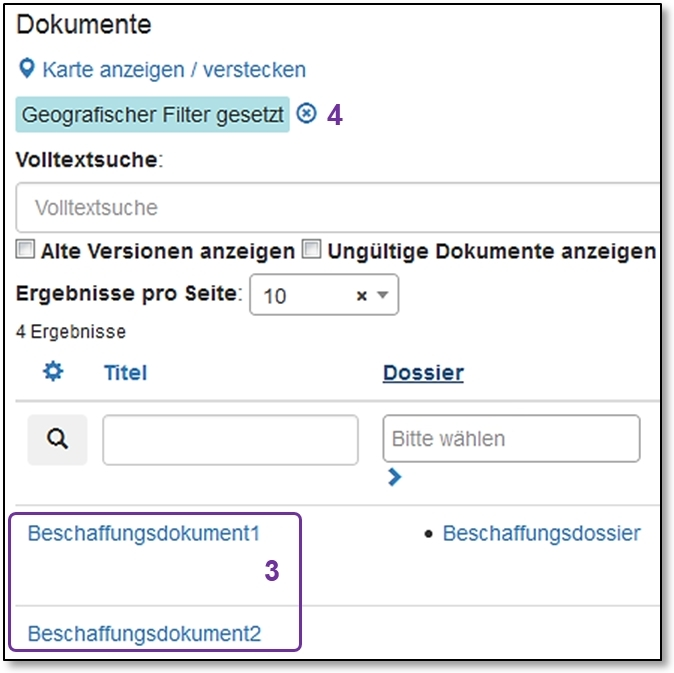
\includegraphics[height=60mm]{../chapters/11_Dokumentenablage/pictures/11-2-3_GeoBereichResult.jpg}
  \end{center}
  \vspace{-20pt}
  % \caption{Geografische Bereiche filtern}
  \vspace{-10pt}
\end{wrapfigure}
'Filtre géographique défini' s'affiche au dessus des champs de recherche / filtrage. Seuls les documents ayant des coordonnées géographiques proches s'affichent. Dans cet exemple, deux document sont listés. Ce sont les deux documents indiqués par des repères sur la carte dans la prise d'écran précédente \col{(3)}. Il s'agit des deux documents des résultats de recherche. Pour enlever le filtre géographique, cliquez sur la petite croix près de 'Filtre géographique défini' \col{(4)}. Cliquez ensuite sur le symbole de loupe \includegraphics[height=12pt]{/Icons/Lupe.jpg} pour afficher la liste de résultats non filtrée.

\subsubsection{Travailler avec les documents chargés}
\label{bkm:Ref442801819}

\begin{figure}[H]
\center{\includegraphics[width=1\linewidth]{../chapters/11_Dokumentenablage/pictures/11-2-4_FunktionenHochgDateien.jpg}}
\caption{Options pour les documents chargés}
% \label{fig:speciation}
\end{figure}

Vous pouvez chercher des documents dans l'aperçu des documents (voir chapitre \ref{bkm:Ref443047823}). Cliquez sur le titre du document désiré (police bleue) \col{(1)} pour visualiser les différentes options. Cliquez sur le titre à nouveau pour masquer les options.

Si le document est associé à Google Maps, cliquez sur le symbole de repère \includegraphics[height=12pt]{/Icons/Nadelsymbol.jpg} \col{(2)} pour naviguer directement au lieu du document sur la carte. Le symbole de repère est uniquement visible si un lien à Google Maps existe (voir chapitre \ref{bkm:Ref442545553}). La fenêtre suivante s'ouvre :

\begin{figure}[H]
\center{\includegraphics[width=0.5\linewidth]{../chapters/11_Dokumentenablage/pictures/11-2-4_DokAufGoogleMaps.jpg}}
% \caption{Das Menü in CUBE PA}
% \label{fig:speciation}
\end{figure}

Depuis cette fenêtre, vous avez la possibilité d'ouvrir la prévisualisation du document, de télécharger le document, ou d'afficher la saisie du document. Cliquez sur la croix dans le coin supérieur droit de la fenêtre pour la fermer. \newline

Cliquez sur le symbole de flèche \includegraphics[height=12pt]{/Icons/Pfeil_rechts.jpg} \col{(3)} pour prévisualiser le document dans l'aperçu des documents, dans la mesure où le format du fichier est supporté. Cliquez sur la flèche \includegraphics[height=12pt]{/Icons/Pfeil_unten.jpg} à nouveau pour fermer la prévisualisation. Plus d'informations sur la prévisualisation sont données plus bas.\newline

Vous pouvez également directement télécharger le document \includegraphics[height=12pt]{/Icons/download.jpg} \col{(4)}, visualiser la saisie du document \includegraphics[height=12pt]{/Icons/Lupe.jpg} \col{(5)} ou modifier la saisie du document \includegraphics[height=12pt]{/Icons/Bearbeiten.jpg} \col{(6)}. \newline

Pour modifier un document en ligne, il doit être extrait avec le symbole \includegraphics[height=12pt]{/Icons/Auschecken.jpg} \col{(7)}. La procédure est décrite dans les détails au chapitre \ref{bkm:Ref442776572}. Cliquez sur le symbole de drapeau gris \includegraphics[height=12pt]{/Icons/DokuFlag_grau.jpg} \col{(8)} pour ajouter un document à vos favoris. Le symbole devient rouge et le document est ajouté à votre aperçu personnel (voir chapitre \ref{bkm:Ref132000001}). Cliquez à nouveau sur le symbole rouge \includegraphics[height=12pt]{/Icons/DokuFlag_rot.jpg} pour enlever le document de vos favoris. \newline


\textbf{Traitement des liens :}

Si le document consiste en un lien au lieu d'un fichier, les options sont légèrement différentes :

\begin{figure}[H]
\center{\includegraphics[width=1\linewidth]{../chapters/11_Dokumentenablage/pictures/11-2-4_Link_verwenden.jpg}}
\caption{Ouvrir un lien}
% \label{fig:speciation}
\end{figure}

Le symbole de lien \includegraphics[height=12pt]{/Icons/Link.jpg} \col{(1)} vous permet d'ouvrir le lien sauvegardé. Cliquez sur le symbole de favoris \includegraphics[height=12pt]{/Icons/DokuFlag_grau.jpg} \col{(2)} pour ajouter le lien à vos favoris afin qu'il apparaisse dans votre aperçu personnel. Vous pouvez également visualiser ou modifier la saisie du lien. Les options manquantes sont les options 'télécharger' et 'extraire'.


\pagebreak
\subsubsection{Visualiser la saisie d'un document}
\label{bkm:Ref443047930}

\begin{wrapfigure}[18]{l}{9.5cm}
\vspace{-15pt}
\includegraphics[height=105mm]{../chapters/11_Dokumentenablage/pictures/11-2-5_Dokumentenansicht.jpg}
% \caption{Status ändern}
\end{wrapfigure}

Quand vous cliquez sur le symbole de loupe \includegraphics[height=12pt]{/Icons/Lupe.jpg}, la saisie du document est ouverte en mode de visualisation. A côté du titre \col{(1)}, toutes les informations (par exemple auteur(s), tags ajoutés lors du chargement ou de la modification du document (voir \ref{bkm:Ref442778397}), etc.) sont affichées. Quand une information manque, le champ correspondant est soit vide soit non affiché. La version du document, l'horodatage, et l'utilisateur qui a modifié le document sont affichés en-dessous du titre \col{(2)}. \newline

Pour télécharger le document, cliquez le symbole de téléchargement \includegraphics[height=12pt]{/Icons/Download.jpg} ou le nom du fichier \col{(3)}. La fenêtre de téléchargement usuelle de votre navigateur s'affichera et vous pouvez choisir d'ouvrir ou de sauvegarder le document. Cliquez sur le symbole d'envoi \includegraphics[height=12pt]{/Icons/Versandsymbol.jpg} \col{(4)} pour envoyer le fichier par courriel à une personne de votre choix (voir chapitre \ref{bkm:Ref201701127} pour plus d'informations). Cliquez sur le symbole de panier à documents \includegraphics[height=12pt]{/Icons/shoppingcart_g.jpg} \col{(5)} pour ajouter le document au panier. La couleur du symbole passe au rouge lorsque le document est dans le panier : \includegraphics[height=12pt]{/Icons/shoppingcart_r.jpg}. Cliquez à nouveau sur le symbole pour enlever le document du panier. La fonction du panier à documents est décrite au chapitre \ref{bkm:Ref201705445}. \newline

Cliquez sur le symbole de favoris \includegraphics[height=12pt]{/Icons/DokuFlag_grau.jpg} \col{(6)} pour afficher le document dans votre aperçu personnel. La couleur du symbole passe au rouge lorsque le document est ajouté à vos favoris : \includegraphics[height=12pt]{/Icons/DokuFlag_rot.jpg}. Cliquez sur le symbole rouge pour enlever le document de votre aperçu personnel. \newline

'Lien statique à la dernière version du fichier' \col{(7)} est un lien que vous pouvez envoyer par e-mail par exemple, tout en restant assuré que le destinataire sera toujours dirigé vers la dernière version du document.

Les premières pages du document sont affichées en vue réduite sous 'Prévisualisation' \col{(8)}.

\vspace{\baselineskip}

Cliquez sur une des pages prévisualisées \col{(9)} pour ouvrir la page dans le mode de prévisualisation. Cliquez sur la croix grise \includegraphics[height=12pt]{/Icons/X_Button.jpg} \col{(a)} dans le coin droit supérieur de la prévisualisation pour la fermer. Cliquez \includegraphics[height=11pt]{/Icons/Weiter.jpg} et \includegraphics[height=11pt]{/Icons/Zurueck.jpg} \col{(b)} pour naviguer les pages du document. Le nombre de pages \col{(c)} est affiché sous les boutons de navigation. Vous pouvez tourner les pages de 90° avec le symbole 90° \includegraphics[height=12pt]{/Icons/90Grad.jpg} \col{(d)}.

\begin{figure}[H]
\center{\includegraphics[width=1\linewidth]{../chapters/11_Dokumentenablage/pictures/11-2-5_Dokumentenvorschau.jpg}}
\caption{Prévisualisation d'un document}
% \label{fig:speciation}
\end{figure}

\textbf{Options supplémentaires dans le mode de visualisation :}

\begin{figure}[H]
\center{\includegraphics[width=1\linewidth]{../chapters/11_Dokumentenablage/pictures/11-2-5_Dokumentenoptionen.jpg}}
\caption{Options additionnelles pour documents chargés}
% \label{fig:speciation}
\end{figure}

Dans le champs 'Extraire fichier' \includegraphics[height=12pt]{/Icons/Auschecken.jpg} \col{(1)}, la dernière version du fichier peut être extraite (voir chapitre \ref{bkm:Ref442780171}). Si le document est classé dans un dossier, cliquez sur le titre du dossier \col{(2)} pour l'ouvrir. Un document peut être classé dans plusieurs dossiers. \newline 

\vspace{\baselineskip}

Sous 'Historique', cliquez sur le symbole de flèche \includegraphics[height=12pt]{/Icons/Pfeil_rechts.jpg} \col{(3)} et les modifications du document s'affichent.

\begin{figure}[H]
\center{\includegraphics[width=1\linewidth]{1125_Aenderungshistorie.jpg}}
\caption{Visualisation de l'historique d'un document}
% \label{fig:speciation}
\end{figure}

Une liste avec les modifications s'affiche. Les modifications des données du document (par exemple, auteurs, tags) et les modifications du document lui-même (nouvelles versions) sont inclues dans la liste. Cliquez sur le symbole de téléchargement \includegraphics[height=12pt]{/Icons/Download.jpg} \col{(6)} pour télécharger une ancienne version du document ou sur le symbole de loupe \includegraphics[height=12pt]{/Icons/Lupe.jpg} \col{(5)} pour visualiser une ancienne version du document. \newline

\begin{wrapfigure}[7]{r}{6cm}
\vspace{-15pt}
\includegraphics[height=40mm]{1125_DokumentAeltereVersion.jpg}
% \caption{Status ändern}
\end{wrapfigure}
Si vous ouvrez une ancienne version d'un document, l'avertissement \textcolor{red}{'Cette version n'est pas la dernière version de ce document!'} apparaît dans l'aperçu de ce document. Si vous téléchargez le document dans le champ 'Fichier', vous n'accédez pas à la dernière version du document, mais à la version ancienne sélectionnée et affichée.

\begin{wrapfigure}[7]{r}{6cm}
% \vspace{-15pt}
\includegraphics[height=35mm]{1125_DokumentBearbeiten.jpg}
% \caption{Status ändern}
\end{wrapfigure}
Pour modifier les informations d'un document ou pour charger une nouvelle version d'un document, cliquez sur le symbole de modification en haut à gauche \includegraphics[height=12pt]{/Icons/Bearbeiten.jpg} \col{(1)}. Le symbole de liste \includegraphics[height=12pt]{/Icons/Listensymbol_zurueck.jpg} \col{(2)} vous permet de retourner à l'aperçu des documents. (Dans la visualisation d'une ancienne version d'un document, le symbole de modification n'est pas disponible. Vous pouvez cliquer sur le symbole de liste \includegraphics[height=12pt]{/Icons/Listensymbol_zurueck.jpg} pour retourner à l'aperçu des documents.)

\vspace{\baselineskip}

\textbf{Détails à propos de l'historique} \\
Toutes les modifications sont enregistrées dans l'historique. D'une part, l'historique enregistre quand un nouveau document (une version révisée) est chargé. D'autre part, les modifications des métadonnées sont aussi enregistrées dans l'historique, sans générer une nouvelle version du document (voir chapitre \ref{bkm:Ref442863508}).

\begin{figure}[H]
\center{\includegraphics[width=1\linewidth]{../chapters/11_Dokumentenablage/pictures/11-2-5_AenderungshistorieUebersicht.jpg}}
\caption{L'aperçu de l'historique d'un document}
% \label{fig:speciation}
\end{figure}

\col{(1)} Dans l'historique, la version du document actuellement ouverte dans le mode de visualisation est affichée avec en caractères gras. Vous pouvez également voir de quelle version du document il s'agit. Les saisies différentes sont séparées par des lignes \col{(2)}. Tous les changements sont enregistrés. Première saisie : Un nouveau fichier a été chargé et une description (métadonnée) a été ajoutée. Deuxième saisie : Le document a seulement été ajouté au dossier d'acquisition. Vous pouvez voir à quelle heure et par qui les modifications ont été effectuées. Pour ouvrir une prévisualisation de la dernière version ou d'une ancienne version du document, cliquez sur le symbole de flèche \includegraphics[height=12pt]{/Icons/Pfeil_rechts.jpg} \col{(3)}. Cliquez sur une des pages pour l'afficher en grand. Vous avez la possibilité de naviguer les pages du document ou de tourner les pages de 90°. Cliquez sur la croix \includegraphics[height=12pt]{/Icons/X_Button.jpg} en haut à droite pour fermer la prévisualisation en grand format. Cliquez sur le symbole de flèche (pointant vers le bas \includegraphics[height=12pt]{/Icons/Pfeil_unten.jpg}) pour fermer la petite prévisualisation.

Dans l'historique, vous pouvez télécharger la dernière version ou une ancienne version d'un document en cliquant sur le symbole de téléchargement \includegraphics[height=12pt]{/Icons/download.jpg} \col{(4)}. Utilisez le symbole de loupe \includegraphics[height=12pt]{/Icons/Lupe.jpg} \col{(5)} pour ouvrir la version correspondante (ancienne) du document en mode de visualisation. Vous avez aussi la possibilité de modifier les métadonnées d'une ancienne version. Pour ce faire, cliquez sur le symbole de modification \includegraphics[height=12pt]{/Icons/Bearbeiten.jpg} \col{(6)}. Avant de modifier, assurez-vous d'avoir ouvert la bonne version.

\vspace{\baselineskip}

\textbf{Remarque :} La modification d'anciennes versions de documents (métadonnées, droits d'accès) est uniquement possible en passant par l'historique, comme décrit ci-dessus.

\pagebreak

\textbf{Charger une nouvelle version d'un document}

\vspace{\baselineskip}

\begin{wrapfigure}[13]{r}{6cm}
\vspace{-35pt}
\includegraphics[height=100mm]{1125_DokumentBearbeitenFelder.jpg}
% \caption{Status ändern}
\end{wrapfigure}
Dans le mode de modification, vous pouvez compléter les informations d'un document (voir chapitre \ref{bkm:Ref442787515}). Pour charger une nouvelle version d'un document, cliquez sous 'Fichier' sur 'Recherche' \col{(1)} et choisissez le fichier désiré. En cas de besoin, d'autres saisies (métadonnées) peuvent être modifiées.

\vspace{\baselineskip}

Quand toutes les saisies nécessaires ont été faites, cliquez sur 'Accepter' \includegraphics[height=12pt]{/Icons/B_Uebernehmen.jpg} en bas à gauche pour charger le document et enregistrer les saisies. L'ancienne version (document et métadonnées) reste enregistrée et peut être accédée à tout moment dans l'historique du document.

\vspace{\baselineskip}
\vspace{\baselineskip}

\textbf{Remarque :} Si plusieurs versions d'un document sont classées dans un même dossier, seule la dernière version sera inclue dans le dossier (ceci se fait automatiquement). Ceci doit être spécialement pris en compte lors de chargement de nouvelles versions de documents. Si par exemple une nouvelle version d'un document ne doit plus être classée dans un certain dossier, la saisie du dossier doit être enlevée en chargeant le document (en cliquant sur l''X' dans le champ 'Dossier' \col{(2)}. De cette manière, les anciennes versions du document ne seront pas "écrasées" dans le dossier.

\begin{figure}[H]
\center{\includegraphics[width=1\linewidth]{1125_DokEintragLoeschen.jpg}}
\caption{Suppression de la saisie d'un dossier}
% \label{fig:speciation}
\end{figure}


\subsubsection{Panier à documents}
\label{bkm:Ref201705445}
% Neues Kapitel

Le panier à documents est similaire à un panier d'achats dans un magasin en ligne. Le panier à documents favorise plusieurs fonctions, comme télécharger des documents dans un fichier zip, les envoyer directement dans un courriel, ou les envoyer à un centre d'impression. Il est donc possible d'ajouter un nombre donné de documents au panier à documents pour ensuite utiliser la fonction désirée sur tous les documents du panier.

\vspace{\baselineskip}

Procédez comme suit :

\begin{figure}[H]
\center{\includegraphics[width=1\linewidth]{../chapters/11_Dokumentenablage/pictures/11-dkorb_Dokumentenkorb_Uebersicht1.jpg}}
\caption{Utiliser le panier à documents}
% \label{fig:speciation}
\end{figure}

Utilisez la recherche plein texte ou le filtre, ou parcourez les documents pour trouver le document que vous voulez ajouter au panier. Sélectionnez le document en cochant la case correspondante \col{(1)}. Répétez ces étapes jusqu'à ce que vous aurez choisi tous les documents avec lesquels vous avez besoin de travailler. Les options disponibles s'affichent au-dessus de la liste \col{(2)}. Vous pouvez également utilisez ces options pour des documents individuels ; elles apparaissent aussi sous le titre d'un document si vous cliquez dessus \col{(8)}. \\
En cliquant sur le symbole de panier à documents \includegraphics[height=12pt]{/Icons/dk_korb_b.jpg} \col{(3)}, les options suivantes s'affichent : vous pouvez soit vider la sélection (enlever tous les documents sélectionnés du panier) \col{(a)} ou afficher la sélection (liste de tous les documents sélectionnés dans le panier) \col{(b)} :
\begin{figure}[H]
\center{\includegraphics[width=.25\linewidth]{../chapters/11_Dokumentenablage/pictures/11-dkorb_Auswahl.jpg}}
% \caption{Weitere Optionen}
% \label{fig:speciation}
\end{figure}
 
Cliquez sur le symbole de favoris \includegraphics[height=12pt]{/Icons/dk_flag_b.jpg} \col{(4)} et tous les documents sélectionnés seront affichés en tant que favoris dans votre aperçu personnel. \\
Cliquez sur le symbole de téléchargement \includegraphics[height=12pt]{/Icons/dk_download.jpg} \col{(5)} pour télécharger tous les documents du panier dans un fichier zip. Si vous voulez envoyer les documents par courriel, cliquez sur le symbole d'envoi \includegraphics[height=12pt]{/Icons/dk_senden.jpg} \col{(6)}. Vous trouverez plus d'informations dans le chapitre \ref{bkm:Ref201701127} (Envoi de documents par courriel). Vous pouvez également envoyer ces documents en version papier. Pour ce faire, cliquez sur le symbole d'imprimante \includegraphics[height=12pt]{/Icons/dk_drucken.jpg} \col{(7)}. Vous trouverez plus d'informations à ce sujet dans le chapitre \ref{bkm:Ref20170609127} (Demandes d'impressions aux centres d'impression).

\vspace{\baselineskip}

Si le panier à documents ne contient qu'un seul document, des options supplémentaires seront disponibles :

\begin{figure}[H]
\center{\includegraphics[width=.8\linewidth]{../chapters/11_Dokumentenablage/pictures/11-dkorb_weitereOptionen.jpg}}
\caption{Otpions supplémentaires}
% \label{fig:speciation}
\end{figure}

En plus des options décrites ci-dessus, le symbole de loupe \includegraphics[height=12pt]{/Icons/dk_lupe.jpg} \col{(1)} vous permet d'afficher les détails du document sélectionné, le symbole de modification \includegraphics[height=12pt]{/Icons/dk_bearb.jpg} \col{(2)} vous permet de modifier le document, le symbole d'épingle \includegraphics[height=12pt]{/Icons/dk_nadel.jpg} \col{(3)} vous permet d'attribuer le document à un emplacement Google Maps, et le symbole d'extraction \includegraphics[height=12pt]{/Icons/dk_auschecken.jpg} \col{(4)} vous permet d'extraire le document. Ces boutons correspondent aux options qui apparaissent sous le titre d'un document dans la liste de documents.

\vspace{\baselineskip}

\textbf{Remarque :} Si la sélection est affichée par le moyen du symbole de panier à documents, le symbole devient rouge \includegraphics[height=12pt]{/Icons/dk_korb_r.jpg}. De même, si vous cliquez sur le symbole de favoris pour la sélection, ce dernier devient rouge aussi \includegraphics[height=12pt]{/Icons/dk_flag_r.jpg} \col{(1)} :

\begin{figure}[H]
\center{\includegraphics[width=.75\linewidth]{../chapters/11_Dokumentenablage/pictures/11-dkorb_Dokumentenkorb_Uebersicht2.jpg}}
\caption{Afficher la sélection du panier à documents / Arrêter l'affichage}
% \label{fig:speciation}
\end{figure}

\textbf{Remarque :} Cliquez sur la croix \includegraphics[height=12pt]{/Icons/FilterLoeschen_b.jpg} \col{(2)} pour arrêter l'affichage. 

\vspace{\baselineskip}

\textbf{Description des options :}

\subsubsection{Envoi de documents par courriel}
\label{bkm:Ref201701127}
% Neues Kapitel

Vous pouvez envoyer des documents en tant que pièces jointes à une personne de votre choix directement depuis la liste de documents. Pour assurer la transparence et la traçabilité, l'envoi de documents est enregistré dans l'historique des documents.

Cliquez sur le symbole d'envoi \includegraphics[height=12pt]{/Icons/Versandsymbol.jpg} pour envoyer tous les documents sélectionnés à une ou plusieurs adresses mail. Vous pouvez toujours enlever les documents que vous ne voulez pas inclure dans le courriel avant de l'envoyer.

\begin{figure}[H]
\center{\includegraphics[width=1\linewidth]{../chapters/11_Dokumentenablage/pictures/11-dkorb_Dok_versenden}}
\caption{Envoi de documents}
% \label{fig:speciation}
\end{figure}

Saisi de destinataires \col{(1)} : Dans le champ 'Destinataires', saisissez une ou plusieurs adresses mail. Séparez les adresses par un point virgule ou un espace.
Dans le champ 'Message' \col{(2)}, saisissez les informations à envoyer au destinataire ou destinataires. Tous les documents sélectionnés qui seront envoyés au destinataire ou destinataires dont affichés. Vous pouvez toujours enlever des documents avant l'envoi en cliquant sur le symbole de croix \includegraphics[height=12pt]{/Icons/blKreuzchen.jpg} \col{(3)}. La taille totale des pièces jointes est affichée en bas de la liste \col{(4)}. Une fois toutes les informations saisies, cliquez sur 'Envoyer' \col{(5)} pour envoyer les documents.

\vspace{\baselineskip}

Une message de confirmation s'affiche, et montre les destinataires du courriel avec les documents envoyés :

\begin{figure}[H]
\center{\includegraphics[width=.4\linewidth]{../chapters/11_Dokumentenablage/pictures/11-dkorb_Sendebestaetigung}}
\caption{Confirmation d'envoi}
% \label{fig:speciation}
\end{figure}

Vous recevrez également un courriel indiquant quels documents ont été envoyés à quels destinataires. Si un courriel n'a pas pu être envoyé à une destinataire, ceci est aussi indiqué.

\vspace{\baselineskip}

\subsubsection{Télécharger les documents dans un fichier zip}
% Neues Kapitel

Vous pouvez télécharger tous les documents sélectionnés dans le panier à documents dans un fichier zip. Pour ce faire, cliquez sur le symbole de téléchargement dans les options du panier à documents.

\vspace{\baselineskip}

La fenêtre de téléchargement de votre navigateur s'affiche. Choisissez si vous voulez ouvrir le fichier zip dans l'explorateur Windows ou le sauvegarder sur votre ordinateur :

\begin{figure}[H]
\center{\includegraphics[width=.5\linewidth]{../chapters/11_Dokumentenablage/pictures/11-dkorb_DokDownload}}
\caption{Télécharger des documents dans un fichier zip}
% \label{fig:speciation}
\end{figure}

\subsubsection{Demandes d'impressions aux centres d'impression}
\label{bkm:Ref20170609127}
% Neues Kapitel

Vous pouvez envoyer des plans directement depuis la liste de documents à un centre d'impression pour une livraison directe des plans imprimés. Plusieurs plans peuvent être livrés à différents destinataires dans le cadre d'une demande. L'exécution se déroule séparément pour chaque destinataire (nombre d'exemplaires, versions papier/électroniques).

\vspace{\baselineskip}

Procédez comme suit pour envoyer des plans par l'intermédiaire de centres d'impression : Comme décrit ci-dessus, sélectionnez tous les documents / plans nécessaires et ajoutez-les au panier à documents. Affichez la sélection du panier à documents et enlevez les documents dont vous n'avez pas besoin \includegraphics[height=12pt]{/Icons/checkbox_markiert.jpg} $ > $ \includegraphics[height=12pt]{/Icons/checkbox_leer.jpg} pour mettre à jour la sélection du panier. Une fois tous les documents / plans sélectionnés, cliquez sur le symbole d'imprimante \includegraphics[height=12pt]{/Icons/printer.jpg} dans le panier à documents. La fenêtre suivante s'affiche :

\begin{figure}[H]
\center{\includegraphics[width=1\linewidth]{../chapters/11_Dokumentenablage/pictures/11-dkorb_ReproDialog1.jpg}}
\caption{Fenêtre 'Informations générales' pour livraison de plans}
% \label{fig:speciation}
\end{figure}

Remplissez les champs de saisie suivants :

\textbf{Projet :} Ceci est un champ obligatoire. Sélectionnez le projet correspondant de la liste de projets prédéfinis. \\
\textbf{Sous-projet / Objet :} Ceci est un champ de texte libre pour toute information additionnelle au projet. \\
\textbf{Centre d'impression :} Ceci est un champ obligatoire. Tous les centres d'impression définis dans les paramètres pas défaut (configuration) peuvent être sélectionnés ici pour la livraison des plans. \\
\textbf{Priorité :} Ceci est un champ obligatoire. Vous pouvez choisir un de trois niveaux de priorité :
\begin{figure}[H]
\center{\includegraphics[width=1\linewidth]{../chapters/11_Dokumentenablage/pictures/11-dkorb_ReproPrio}}
\caption{Sélection de priorité pour la livraison de plans}
% \label{fig:speciation}
\end{figure}
Vous devrez prendre en compte que la livraison dépendra du moment de la commande. Pour plus de détails, prenez contact avec les entités responsables. \\
\textbf{Délai :} Ceci est un champ obligatoire. La date de livraison est déterminée automatiquement selon le niveau de priorité de la commande est peut être ultérieurement modifée. \\
\textbf{Objectif :} Vous pouvez choisir un ou plusieurs objectifs d'une liste prédéfinie. Ces derniers apparaîtront sur le bulletin de livraison des destinataires.
\begin{figure}[H]
\center{\includegraphics[width=1\linewidth]{../chapters/11_Dokumentenablage/pictures/11-dkorb_ReproZweck}}
\caption{Saisie de l'objectif pour le bulletin de livraison}
% \label{fig:speciation}
\end{figure}
\textbf{Message aux destinataires :} Ceci est un champ de texte libre où vous pouvez saisir des informations nécessaires pour le ou les destinataires. \\
\textbf{Message au centre d'impression :} Ce message sera visible pour le centre d'impression après que vous avez placé la commande. \\
\textbf{Pièces jointes :} Vous pouvez ajouter des spécifications pour chaque document de la sélection qui est maintenant prêt pour la livraison. Cliquez sur le titre du document / plan en bleu pour l'ouvrir ou le sauvegarder sur votre ordinateur.
En général, les dimensions du plan sont basées sur le fichier PDF. Vous pouvez cependant toujours changer les dimensions et demander un autre format au centre d'impression. De plus, vous pouvez spécifier si vous voulez que les plans soient imprimés en noir et blanc ou en couleur. Vous pouvez également préciser la finition des documents imprimés à livrer à un chantier ou à un bureau.
Une fois toutes les informations nécessaires saisies, cliquez sur 'Continuer aux détails du destinataire' :

\begin{figure}[H]
\center{\includegraphics[width=1\linewidth]{../chapters/11_Dokumentenablage/pictures/11-dkorb_ReproDialog2.jpg}}
\caption{Fenêtre 'Détails du destinataire' pour livraison de plans}
% \label{fig:speciation}
\end{figure}

Dans cette fenêtre vous pouvez choisir un ou plusieurs destinataires pour la livraison de plans. Procédez comme suit : Sélectionnez la personne désirée dans le menu déroulant 'Ajouter destinataires'. Répétez cette étape jusqu'à ce que vous aurez ajouter tous les destinataires auxquels vous voulez faire livrer des plans. Une fois que vous avez cliqué sur le symbole plus (ajouter), la personne est ajoutée au bas de la fenêtre. vous pouvez également définir des spécifications additionnelles, comme par exemple le nombre d'exemplaires nécessaire par destinataire et si le destinataire doit recevoir une version papier (Imprimé) et / ou une version électronique par courriel (Électronique). \\
Vous pouvez aussi envoyer des messages personnalisés aux différents destinataires (e-mail / bon de livraison) \col{(2)}. Si des messages sont saisis ici, le message général de la première page de la fenêtre sera écrasé (voir aussi l'indication en cliquant sur \includegraphics[height=12pt]{/Icons/Info_blau.jpg}. \col{(2)}\\
Le symbole de poubelle \includegraphics[height=12pt]{/Icons/Muelltonne.jpg} \col{(3)} vous permet d'enlever des destinataires. Si des destinataires déjà sélectionnés sont ajoutés à la liste au moyen du menu déroulant 'Ajouter destinataires' \col{(1)}, le message suivant apparaît :

\begin{figure}[H]
\center{\includegraphics[width=.5\linewidth]{../chapters/11_Dokumentenablage/pictures/11-dkorb_Meldung_doppeltePerson.jpg}}
\caption{Alerte : Le destinataire existe déjà}
% \label{fig:speciation}
\end{figure}

\vspace{\baselineskip}

Si vous avez besoin de faire des changements ou simplement de vérifier la section 'Informations générales', cliquez sur 'Retour aux informations générales'. Quand vous avez tout vérifié, cliquez sur 'Envoyer commande'. Le bulletin de livraison est affiché et les courriels correspondants sont envoyés. Le centre d'impression reçoit la commande par courriel avec un lien vers CUBE PA pour pouvoir exécuter la commande. Quand le centre d'impression a exécuté la commande, cette dernière est marquée comme 'terminée' par le centre d'impression et la personne qui a passé la commande est avisée.

\vspace{\baselineskip}

Une fois la commande passée, celle-ci s'affiche dans l'aperçu personnel de la personne (utilisateur CUBE PA) qui l'a placée (CUBE PA user). De même, une fois que le centre d'impression a marqué la commande comme 'terminée', ceci est affiché dans l'aperçu personnel.

\vspace{\baselineskip}

\textbf{Remarque importante :} Si vous cliquez sur le symbole de la croix \includegraphics[height=12pt]{/Icons/X_BUtton.jpg} (en haut à droite) de la fenêtre de livraison de plans pendant que vous êtes en train de saisir des données, toutes ces données / saisies seront perdues. Les documents /plans restent dans le panier à documents et vous pouvez redémarrer le processus avec une nouvelle commande.

\subsubsection{Gérer les droits d'accès aux documents}
\label{bkm:Ref442869495}

Vous pouvez choisir pour chaque document qui peut lire, modifier, et/ou supprimer le document (la suppression de documents est pour l'instant pas possible). Vous pouvez attribuer des droits d'accès pour un ou plusieurs groupes ou pour un ou plusieurs utilisateurs :

\begin{figure}[H]
\center{\includegraphics[width=1\linewidth]{../chapters/11_Dokumentenablage/pictures/11-berecht_Rechte.jpg}}
\caption{Nouveau document : Droits d'accès}
% \label{fig:speciation}
\end{figure}

Vous devez attribuer au moins un droit d'accès par document. Si aucun droit d'accès n'est sélectionné / attribué, le message d'erreur suivant apparait :

\begin{figure}[H]
\center{\includegraphics[width=.6\linewidth]{../chapters/11_Dokumentenablage/pictures/11-berecht_Fehlermeldung.jpg}}
\caption{Message d'erreur droits d'accès}
% \label{fig:speciation}
\end{figure}

Cliquez sur 'OK' pour retourner à la saisie.

\vspace{\baselineskip}

Cliquez sur le symbole plus (ajouter) \includegraphics[height=12pt]{/Icons/Pluszeichen.jpg} \col{(1)} pour attribuer des droits d'accès au document. Cliquez sur le symbole de liste \includegraphics[height=12pt]{/Icons/Listensymbol_zurueck.jpg} \col{(2)} pour retourner à l'aperçu des documents.

\vspace{\baselineskip}

Quand vous cliquez sur le symbole plus (ajouter) \includegraphics[height=12pt]{/Icons/Pluszeichen.jpg} \col{(1)}, le masque de saisie suivant apparaît danslequel vous pouvez accéder aux droits d'accès :

\begin{figure}[H]
\center{\includegraphics[width=1\linewidth]{../chapters/11_Dokumentenablage/pictures/11-berecht_RechteVergeben.jpg}}
\caption{Attribuer des droits d'accès}
% \label{fig:speciation}
\end{figure}

Vous pouvez attribuer les droits d'accès par défaut au document. Pour ce faire, cocher la case 'Utiliser les droits d'accès par défaut' \col{(1)}. Si vous utilisez les droits d'accès par défaut, vous (parmi d'autres) recevrez les droits d'accès complets au document que vous avez créé. De plus, des groupes prédéfinis auront également les droits d'accès au document. (Dans la gestion des utilisateurs, des groupes peuvent être définis, pour lesquels les droits d'accès aux documents sont automatiquement attribués lorsque la case 'Utiliser les droits d'accès par défaut' est cochée. Ces paramètres sont définis par l'utilisateur de référence ('poweruser').)

\begin{figure}[H]
\center{\includegraphics[width=1\linewidth]{../chapters/11_Dokumentenablage/pictures/11-berecht_Standard-Rechte.jpg}}
\caption{Attribuer les droits d'accès}
% \label{fig:speciation}
\end{figure}

Vous pouvez modifier les droits d'accès à tout moment. Le symbole plus (ajouter) \includegraphics[height=12pt]{/Icons/Pluszeichen.jpg} \col{(1)} vous permet d'ajouter des groupes / utilisateurs supplémentaires et de définir les droits d'accès : Choisissez un groupe qui peut visualiser / modifier le document (le groupe doit déjà exister) ou choisissez un utilisateur. Cliquez sur la petite flèche \includegraphics[height=12pt]{/Icons/Dropdown.jpg} près de 'Veuillez choisir' ou sur le nom. Un menu déroulant s'affiche et vous pouvez choisir le groupe / l'utilisateur désiré. Sous 'Accès' \col{(2)}, choisissez les droits pour le groupe / l'utilisateur choisi : lire / modifier / supprimer.

\vspace{\baselineskip}

Vous pouvez également modifier ou supprimer des droits d'accès existants pour des groupes / utilisateurs \col{(2)}. Pour supprimer des droits d'accès, cliquez sur le symbole de poubelle \includegraphics[height=12pt]{/Icons/Muelltonne.jpg} \col{(3)} et confirmez le message de sécurité par 'OK'.  \newline

Une fois les changements nécessaires effectués, cliquez sur 'Actualiser'. 

\vspace{\baselineskip}

\textbf{Remarque :} Pour le premier utilisateur / groupe (en général l'utilisateur qui crée le document dans CUBE PA), tous les droits d'accès sont automatiquement cochés. Pour chaque groupe / utilisateur additionnel, seul les droits de lecture sont automatiquement cochés. Ceci peut être modifié à tout moment.


\subsubsection{Modifier documents en ligne / Extraire et réintroduire des documents}
\label{bkm:Ref442780171}\label{bkm:Ref442776572}

Pour modifier le contenu d'un document puis enregistrer une nouvelle version du document dans le classement des documents, suivez les étapes suivantes :

\begin{figure}[H]
\center{\includegraphics[width=.75\linewidth]{../chapters/11_Dokumentenablage/pictures/11-2-7_DokumentAusEinchecken.jpg}}
\caption{Fonctions dans l'aperçu des documents}
% \label{fig:speciation}
\end{figure}

Dans l'aperçu des documents, cliquez sur le titre en bleu du document désiré \col{(1)}. Les options s'affichent. Cliquez sur le symbole d'extraction \includegraphics[height=12pt]{/Icons/Auschecken.jpg} \col{(4)}. Alternativement, vous pouvez extraire le document dans le mode de visualisation du document (accessible par le symbole de loupe \includegraphics[height=12pt]{/Icons/Lupe.jpg} \col{(3)} dans l'aperçu des documents). Le document sera extrait, ouvert, et verrouillé contre les modifications par d'autres utilisateurs. Vous pouvez maintenant directement travailler dans le document.

\begin{wrapfigure}[5]{r}{6cm}
\vspace{-15pt}
\includegraphics[height=30mm]{1127_WordSpeichern.jpg}
% \caption{Status ändern}
\end{wrapfigure}
Pour arrêter la modification, enregistrez le document en cliquant le symbole correspondant dans le programme MS Office \col{(1)} (ici Office 2013 -- en haut à gauche) ou avec le raccourci 'Ctrl+S'. Le document mis à jour sera directement enregistré sur le serveur. Pour continuer à modifier le document ultérieurement, cliquez le symbole \includegraphics[height=12pt]{/Icons/Wolke_blauklein.jpg} \col{(2)} (ouvrir le document extrait) dans l'aperçu des document ou dans le mode de visualisation du document que vous voulez modifier.

\begin{figure}[H]
\center{\includegraphics[width=1\linewidth]{../chapters/11_Dokumentenablage/pictures/11-2-7_DokumentOeffnen.jpg}}
\caption{Ouvrir un document extrait}
% \label{fig:speciation}
\end{figure}

Une fois les modifications terminées et sauvegardées, vous pouvez réintroduire le document 
en cliquant sur le symbole de réintroduction \includegraphics[height=12pt]{/Icons/Einchecken.jpg} \col{(3)} dans l'aperçu des documents ou dans le mode de visualisation du document. Le dernier document enregistré dans le serveur est fixé comme dernière version dans le classement des documents. Les symboles pour ouvrir un document extrait ou réintroduire un document extrait sont uniquement visibles pour les documents qui sont extraits.

\begin{figure}[H]
\center{\includegraphics[width=1\linewidth]{../chapters/11_Dokumentenablage/pictures/11-2-7_DokumentEinchecken.jpg}}
\caption{Réintroduire un document extrait}
% \label{fig:speciation}
\end{figure}

Comme alternative pour la modification de documents en ligne, vous pouvez aussi travailler 'offline'. Pour ce faire, il faut extraire le document comme décrit ci-dessus. Ensuite, il faut enregistrer le document localement sur votre disque dur en utilisant 'Enregistrer sous' dans le programme MS Office. Pour charger le document à nouveau, vous devez d'abord réintroduire le document (voir ci-dessus).
Le dernier document enregistré sur le serveur sera chargé. Comme entre temps, vous avez effectué des modifications localement, vous devez aussi charger le document que vous avez enregistré localement. Ceci peut se faire dans le mode de modification du document (voir chapitres \ref{bkm:Ref442801819} et \ref{bkm:Ref443047930}). \newline

Si vous voulez travailler 'offline', il n'est pas nécessaire d'extraire le document et de le réintroduire après avoir effectué les modifications. Vous pouvez aussi télécharger un document, l'enregistrer localement, le modifier, et puis le charger à nouveau (nouvelle version, voir chapitres \ref{bkm:Ref442801819} et \ref{bkm:Ref443047930}). Par contre, la procédure d'extraction et de réintroduction assure qu'un document ne peut pas être modifié par plusieurs utilisateurs à la fois.

\vspace{\baselineskip}

\textbf{Conseil :} Un document que vous avez extrait apparaît automatiquement dans votre aperçu personnalisé. Vous pouvez directement y ouvrir un document ou le réintroduire. \newline

%\vspace{\baselineskip}

\textbf{Remarque :} La modification de documents en ligne peut se faire avec les programmes MS Office usuels. Les documents sous autres formats (par exemples PDF ou plans CAD) peuvent aussi être extraits, mais ne peuvent pas être modifiés en ligne. La modification de tels documents peut uniquement se faire offline. \newline

% \vspace{\baselineskip}

\textbf{Remarque :} Un document extrait est verrouillé contre les changements par d'autres utilisateurs. Les symboles pour modifier et extraire le document ne seront pas accessibles et un symbole d'avertissement rouge \includegraphics[height=12pt]{/Icons/Warnung_rot.jpg} \col{(1)} apparaît à leur place. Dans le champ 'Extraire document (dernière version)' dans le mode de visualisation du document, un message indique que le document est actuellement extrait \col{(2)}.

\begin{figure}[H]
\center{\includegraphics[width=1\linewidth]{1127_DokumentGesperrt.jpg}}
\caption{Document verrouillé contre les modifications}
% \label{fig:speciation}
\end{figure}

\subsubsection{Utilisation de tags}
\label{bkm:Ref201801219}

L'attribution de tags dans le classement de documents est une fonction centrale qui vous permet de rapidement atteindre des résultats de recherche spécifiques. Les tags / structures de tags sont établis par l'administrateur. Des modifications rétroactives sont que difficilement possibles. Un document peut être attribué plusieurs tags. Dans le chapitre \ref{bkm:Ref442275849} (Recherche selon tags), vous découvrirez davantage d'informations sur la fonction de recherche par tags. \newline

\vspace{\baselineskip}

Lorsque vous ajoutez un document, ou plus tard lorsque vous le modifiez, sélectionnez les tags souhaités. Procédez comme suit : 

\begin{figure}[H]
\center{\includegraphics[width=1\linewidth]{../chapters/11_Dokumentenablage/pictures/11-tags_TagsAuswaehlen.jpg}}
\caption{Sélection de tags}
% \label{fig:speciation}
\end{figure}

Sous 'Tags' \col{(1)}, le symbole de boussole \includegraphics[height=12pt]{/Icons/Ziel.jpg} \col{(2)} vous permet d'afficher et de naviguer la structure de tags. Alternativement, vous pouvez utiliser le champ de saisie \col{(3)} pour saisir le nom d'un tag. Le résultat de recherche s'affiche et se raffine pendant que vous tapez, et vous pouvez sélectionner un des résultats affichés \col{(4)}. Lorsque vous appuyez la touche 'Enter' ou que vous cliquez sur un des résultat, la structure de tags est également affichée :

\begin{figure}[H]
\center{\includegraphics[width=1\linewidth]{../chapters/11_Dokumentenablage/pictures/11-tags_TagsStruktur.jpg}}
\caption{Structure de tags sans et avec saisie de tag}
% \label{fig:speciation}
\end{figure}

Cliquez sur le symbole d'information \includegraphics[height=12pt]{/Icons/Info_Hinweis.jpg} \col{(1)} pour afficher la légende de l'aperçu de tags :

\begin{figure}[H]
\center{\includegraphics[width=1\linewidth]{../chapters/11_Dokumentenablage/pictures/11-tags_Legende.jpg}}
\caption{Légende pour la structure de tags}
% \label{fig:speciation}
\end{figure}

Les flèches \includegraphics[height=12pt]{/Icons/Pfeil_rechts.jpg} vous permettent d'approfondir la structure et les symboles plus \includegraphics[height=12pt]{/Icons/Pluszeichen.jpg} vous permettent d'ajouter des tags au document. Vous pouvez de cette manière ajouter autant de tags que vous le souhaitez. Dans la photo de droite, le résultat de recherche pour le tag 'Logistique' est présenté \col{(2)}. La structure est affichée de telle façon à montrer toutes les branches dans lesquelles ce tag est classé. Ce tag n'est pas automatiquement sélectionné, mais doit être ajouté manuellement en cliquant sur le symbole plus \includegraphics[height=12pt]{/Icons/Pluszeichen.jpg}. Le symbole de triangle \includegraphics[height=12pt]{/Icons/welcheSpalte_sort.jpg} vous permet d'afficher le reste des tags qui sont dans une branche de la structure mais ne faisant pas partie du résultat de recherche. \newline

Lorsque vous avez fini d'ajouter des tags, fermer la fenêtre en cliquant sur la croix en haut à droite \includegraphics[height=12pt]{/Icons/X_Button.jpg}. Vous retournez au masque de modification du document et vous pouvais désormais voir la liste des tags sélectionnés :

\begin{figure}[H]
\center{\includegraphics[width=1\linewidth]{../chapters/11_Dokumentenablage/pictures/11-tags_ausgew_Tags.jpg}}
\caption{Tags sélectionnés}
% \label{fig:speciation}
\end{figure}

Le symbole de croix \includegraphics[height=12pt]{/Icons/Kreuzchen_b.jpg} \col{(1)} vous permet de supprimer des tags choisis.


% bishierher


\subsubsection{Recherche selon tags}
\label{bkm:Ref442275849}

Des tags (ou étiquettes) peuvent être définis pour chaque document. Il devient alors possible de chercher selon des tags spécifiques pour trouver les documents de projets, phases de projet, domaines d'expertise, ou types de documents spécifiques. Une structure de tags (thèmes / catégories de tags et tags attribués à ces thèmes / catégories) est idéalement préalablement établie sur mesure. L'attribution d'un tag à un document est décrite au chapitre \ref{bkm:Ref201801219}.

\begin{figure}[H]
\center{\includegraphics[width=1\linewidth]{../chapters/11_Dokumentenablage/pictures/11-2-8_DokUebersichtTag.jpg}}
\caption{Aperçu des documents - Utilisation du filtre}
% \label{fig:speciation}
\end{figure}

\begin{wrapfigure}[8]{r}{5cm}
\vspace{-10pt}
\includegraphics[height=50mm]{../chapters/11_Dokumentenablage/pictures/11-2-8_DokTagHinzufuegen.jpg}
% \caption{Status ändern}
\end{wrapfigure}
Afin de chercher les documents avec les tags, procédez comme suit : 
Dans le menu à gauche, choisissez l'élément 'Classement des documents' puis le sous-élément 'Documents'. Dans l'aperçu des documents, une liste des documents saisis / chargés est présentée \col{(1)}. Dans la colonne 'Tags', cliquez sur le champ de recherche \col{(2)}. Vous pouvez alors choisir les tags désirés soit en les tapant manuellement dans le champ soit en les sélectionnant dans le menu déroulant \col{(3)}.

\vspace{\baselineskip}

\begin{wrapfigure}[6]{r}{5cm}
\vspace{-30pt}
\includegraphics[height=50mm]{../chapters/11_Dokumentenablage/pictures/11-2-8_TagEingabe.jpg}
% \caption{Status ändern}
\end{wrapfigure}
Vous pouvez choisir simultanément plusieurs tags pour une recherche. Pour ce faire, cliquez à droite du premier tag \col{(4)} dans le champ de saisie \col{(5)} (le tag sera entouré d'un champ gris). Après avoir saisi les tags, cliquez sur le symbole de loupe (à gauche des champs de saisie des filtres) \includegraphics[height=12pt]{/Icons/Lupe_kl.jpg} \col{(6)} ou appuyez sur la touche Entrée. Tous les documents auxquels ces tags sont attribués seront listés.

\vspace{\baselineskip}

\subsubsection{Recherche avancée}

Pour afficher uniquement les documents auxquels tous les tags choisis sont attribués, faites comme suit :

\begin{figure}[H]
\center{\includegraphics[width=0.6\linewidth]{../chapters/11_Dokumentenablage/pictures/11-2-8_TagsFiltern.jpg}}
\caption{Lier les tags avec 'ET' / 'OU'}
% \label{fig:speciation}
\end{figure}

Sous le champ de saisie dans la colonne 'Tags', cliquez sur le symbole \includegraphics[height=12pt]{/Icons/Pfeil_rechts.jpg} \col{(1)} pour afficher la fenêtre de recherche avancée. Dans le champ 'lier' \col{(2)}, choisissez la valeur 'ET' \col{(3)} du menu déroulant. Cliquez ensuite sur le symbole de loupe (à gauche des champs de saisie des filtres) \includegraphics[height=12pt]{/Icons/Lupe.jpg} \col{(4)} ou appuyez sur la touche Entrée. Seuls les documents auxquels tous les tags choisis sont attribués s'affichent. La valeur 'OU' est choisie par défaut, c'est-à-dire que seuls un des tags doit correspondre à la recherche.\newline

Pour exclure certains tags de la recherche, choisissez ces derniers dans le champ 'exclure' \col{(5)}. Vous pouvez choisir plusieurs tags. Cliquez sur le symbole de loupe \includegraphics[height=12pt]{/Icons/Lupe_kl.jpg} et seuls les documents auxquels ces tags ne sont pas attribués seront s'affichent. Les fonctions de recherche avancée 'lier' et 'exclure' peuvent également être combinées.

\vspace{\baselineskip}

Cliquez sur le symbole de flèche \includegraphics[height=12pt]{/Icons/Pfeil_unten.jpg} \col{(6)} pour masquer la fenêtre de recherche avancée.

\vspace{\baselineskip}

\textbf{Remarque :} Cliquez sur la croix bleue \includegraphics[height=12pt]{/Icons/Kreuzchen_b.jpg} près de l'en-tête de la colonne 'Tags' pour supprimer toutes les saisies de tags (réinitialisation du filtre de tags).

\vspace{\baselineskip}

\textbf{Remarque :} Dans le champ de recherche 'Tags', vous pouvez uniquement chercher des tags définis au préalable.

\vspace{\baselineskip}

La fonction de recherche avancée fonctionne aussi avec les dossiers. Les fonctions 'lier' ('ET' / 'OU') et 'exclure' sont identiques à celles de la recherche avancée pour les tags.

\subsubsection{Tags hiérarchiques : Recherche de document dans une 'structure de dossiers'}
\label{bkm:Ref201801849}
% Neues Kapitel

En plus de rechercher des documents par le moyen des tags, il est possible d'établir une 'structure de dossiers' et d'y placer des documents chargés. Ceci permet un usage combiné et optimisé des avantages des deux types de classement : les 'tags' et les 'dossiers'. Les documents peuvent être recherchés à travers un ou plusieurs tags ainsi qu'en navigant la structure hiérarchique du classement des documents. Le même document peut être classifiés et recherchés dans plusieurs 'arbres hiérarchiques' à la fois.

\vspace{\baselineskip}

\textbf{Remarque :} La création de la structure de dossier est expliquée au chapitre de configuration. Il convient de noter que des droits d'accès spécifiques sont requis pour accéder à la configuration. De plus, plusieurs points sont à considérer lors de la création de la structure. La préparation de la structure est une étape cruciale pour un bon futur déroulement. Si vous avez des questions, prenez contact avec votre utilisateur de référence (poweruser) chez Emch+Berger AG Bern.

\vspace{\baselineskip}

En navigant la structure de dossiers, les tags correspondants sont automatiquement fixés dans le filtre 'Tags' :

\begin{figure}[H]
\center{\includegraphics[width=0.6\linewidth]{../chapters/11_Dokumentenablage/pictures/11-htag_Start.jpg}}
\caption{Utiliser la structure de dossiers}
% \label{fig:speciation}
\end{figure}

Une fois une structure de dossiers établie, un onglet avec le titre de la structure apparaît comme montré dans l'image sous \col{(1)}. Cette structure de dossiers est appelée 'Fiches de référence'. Le titre peut être choisi librement. De plus, il est possible d'établir plusieurs structures de dossier. Cliquez sur le titre d'une structure pour afficher le prochain niveau dans la structure \col{(1)} :

\begin{figure}[H]
\center{\includegraphics[width=1\linewidth]{../chapters/11_Dokumentenablage/pictures/11-htag_Nav.jpg}}
\caption{Naviguer la structure de dossiers}
% \label{fig:speciation}
\end{figure}

Cliquez sur 'Systèmes ferroviaires' \col{(1)} pour passer au prochain niveau / sélection. Sous 'Systèmes ferroviaires' se trouvent entre autres les dossiers 'Domaines d'expertise' et 'Pays'. Sélectionnez 'Opération ferroviaire' \col{(2)} dans ce niveau pour aller plus profondément dans la structure de dossiers. Sous 'Opération ferroviaire' vous trouverez le dossier 'Services' et ses tags correspondants. Choisissez par exemple le tag 'Logistique de chantier' \col{(3)} pour pouvoir voir les résultats de votre recherche. Pendant que vous naviguiez la structure de tags, les tags correspondant ont automatiquement été fixés dans le filtre :

\begin{figure}[H]
\center{\includegraphics[width=.75\linewidth]{../chapters/11_Dokumentenablage/pictures/11-htag_Tags.jpg}}
\caption{Résultat du filtre}
% \label{fig:speciation}
\end{figure}

Les tags séclectionnls ont été fixés dans le filtre \col{(1)}. Vous pouvez toujours enlever des tags individuels ou tous les tags en cliquant sur le symbole de croix. La nouvelle recherche avec le filtre adapté s'effectuera quand vous aurez cliqué sur le symbole de loupe \col{(2)}. Cliquez sur le symbole de dossier \includegraphics[height=12pt]{/Icons/Ordner.jpg} \col{(2)} pour ouvrir la structure de dossiers actuelle dans un aperçu : 

\begin{figure}[H]
\center{\includegraphics[width=.75\linewidth]{../chapters/11_Dokumentenablage/pictures/11-htag_Uebersicht.jpg}}
\caption{Aperçu structure de dossiers}
% \label{fig:speciation}
\end{figure}

Vous pouvez maintenant naviguer dans l'aperçu. Vous pouvez fermer des dossiers ouverts \col{(1)} et ouvrir d'autres dossiers \col{(2)}. Cliquez sur la flèche bleue \includegraphics[height=12pt]{/Icons/Pfeil-rechts.jpg} \col{(3)} pour remplir le filtre avec les tags correspondants. Pour fermer la fenêtre avec l'aperçu, cliquez sur le symbole de croix \includegraphics[height=12pt]{/Icons/x_Button.jpg} \col{(4)}.


\pagebreak

\begin{wrapfigure}[5]{r}{6cm}   % [x] Wie manche Zeile soll sich um die Grafik "brechen"
  \vspace{-30pt}      % Grundwert war 20; mit 30 schön oben beim Text ausgerichtet
  \begin{center}
    \includegraphics[height=50mm]{../chapters/11_Dokumentenablage/pictures/11-htag_FilterLoeschen.jpg}
  \end{center}
  \vspace{-20pt}
  \caption{Supprimer un filtre}
  \vspace{-10pt}
\end{wrapfigure}
Dans la structure de dossiers, si vous cliquez sur 'Systèmes ferroviaires' \col{(1)} par exemple, les tags enfants sont enlevés du filtre. Cliquez sur le symbole de filtre à gauche de 'Systèmes ferroviaires' \includegraphics[height=12pt]{/Icons/fOrdner.jpg} \col{(2)} pour enlever tous les tags du filtre.

\vspace{\baselineskip}
\vspace{\baselineskip}
\vspace{\baselineskip}
\vspace{\baselineskip}

\subsubsection{Utiliser le classement des documents avec des appareils mobiles}

Vous pouvez installer CUBE PA comme application sur votre appareil Android ou iPhone. Pour ce faire, ouvrez Google-Play ou l'App store d'Apple pour télécharger l'application.

\vspace{\baselineskip}

\textbf{Remarque :} Veuillez noter que les instructions et prises d'écran suivantes sont basées sur un iPhone / appereil iOS. Pour les appareils Android, certaines fonctionnalités pourraient être légèrement différentes.

\vspace{\baselineskip}

Sous le classement des documents, vous pouvez parcourir et visualiser des documents mains aussi ajouter de nouveaux documents ou photos. Si vos photos disposent de marques GPS, ces dernières seront aussi chargées dans CUBE PA.

\vspace{\baselineskip}

\textbf{Remarque :} Les marques GPS seront aussi traitées lors du chargement de photos d'appareils non mobiles.

\vspace{\baselineskip}

\begin{wrapfigure}[7]{l}{6.5cm}   % [x] Wie manche Zeile soll sich um die Grafik "brechen"
  \vspace{-35pt}      % Grundwert war 20; mit 30 schön oben beim Text ausgerichtet
  \begin{center}
    \includegraphics[width=1\linewidth]{../chapters/11_Dokumentenablage/pictures/11-mob01_Dokumentenablage_oeffnen.jpg}
  \end{center}
  \vspace{-20pt}
  %\caption{Using document management}
  \vspace{-10pt}
\end{wrapfigure}

Connectez-vous à CUBE PA dans l'application mobile. Cliquez sur le symbole de menu en haut à droite \includegraphics[height=12pt]{/Icons/mob_Menu.jpg} puis choisissez 'Classement des documents'.

\vspace{.5cm}

Vous pouvez parcourir, visualiser et envoyer des documents existants dans CUBE PA, ou y charger de nouveaux documents et photos.

\vspace{\baselineskip}

\begin{wrapfigure}[2]{l}{6.5cm}   % [x] Wie manche Zeile soll sich um die Grafik "brechen"
  \vspace{-35pt}      % Grundwert war 20; mit 30 schön oben beim Text ausgerichtet
  \begin{center}
    \includegraphics[width=1\linewidth]{../chapters/11_Dokumentenablage/pictures/11-mob02_Dokumente_anschauen.jpg}
  \end{center}
  \vspace{-20pt}
  % \caption{Die Dokumentenablage verwenden}
  \vspace{-10pt}
\end{wrapfigure}

% \vspace{\baselineskip}

\textbf{Visualiser des documents :} Cliquez sur 'Documents'

\pagebreak

\begin{wrapfigure}[6]{l}{6.5cm}   % [x] Wie manche Zeile soll sich um die Grafik "brechen"
  \vspace{-35pt}      % Grundwert war 20; mit 30 schön oben beim Text ausgerichtet
  \begin{center}
    \includegraphics[width=1\linewidth]{../chapters/11_Dokumentenablage/pictures/11-mob04_Dokumentenuebersicht.jpg}
  \end{center}
  \vspace{-20pt}
  % \caption{Die Dokumentenablage verwenden}
  \vspace{-10pt}
\end{wrapfigure}

Saisissez un mot-clé dans le champ de recherche \col{(2)} puis cliquez sur le symbole de loupe \includegraphics[height=12pt]{/Icons/Lupe_kl.jpg} \col{(3)}. L'affichage est filtré et les résultats de recherche sont listés \col{(4)}. Pour régler d'autres paramètres de filtre, cliquez sur le symbole de filtre \includegraphics[height=12pt]{/Icons/Filter.jpg} \col{(1)}. Des champs de recherche additionnels apparaissent :

\vspace{3.5cm}

\begin{wrapfigure}[5]{l}{6.5cm}   % [x] Wie manche Zeile soll sich um die Grafik "brechen"
  \vspace{-35pt}      % Grundwert war 20; mit 30 schön oben beim Text ausgerichtet
  \begin{center}
    \includegraphics[width=1\linewidth]{../chapters/11_Dokumentenablage/pictures/11-mob05_Filterverwenden.jpg}
  \end{center}
  \vspace{-20pt}
  % \caption{Die Dokumentenablage verwenden}
  \vspace{-10pt}
\end{wrapfigure}

Saisissez les termes de recherche désirés ou connus puis cliquez sur le symbole de loupe \includegraphics[height=12pt]{/Icons/Lupe_kl.jpg}. Les résultats de recherche sont affichés. Pour cacher les paramètres de recherche avancée, cliquez à nouveau sur le symbole de filtre \includegraphics[height=12pt]{/Icons/Filter.jpg} \col{(1)}.

%\vspace{8cm}

\pagebreak

Pour visualiser ou envoyer un document, cliquez d'abord sur le document désiré :

\vspace{\baselineskip}

\begin{wrapfigure}[5]{l}{6.5cm}   % [x] Wie manche Zeile soll sich um die Grafik "brechen"
  \vspace{-35pt}      % Grundwert war 20; mit 30 schön oben beim Text ausgerichtet
  \begin{center}
    \includegraphics[width=1\linewidth]{../chapters/11_Dokumentenablage/pictures/11-mob06_Dokumente_anschauen.jpg}
  \end{center}
  \vspace{-20pt}
  % \caption{Die Dokumentenablage verwenden}
  \vspace{-10pt}
\end{wrapfigure}

Différentes options sont affichées. Par exemple, vous pouvez envoyer une document par e-mail ou l'envoyer à une autre application. Pour visualiser le document sur votre appareil mobile, cliquez sur 'Quick Look' et le document est ouvert.

\vspace{9.5cm}

\begin{wrapfigure}[6]{l}{6.5cm}   % [x] Wie manche Zeile soll sich um die Grafik "brechen"
  \vspace{-35pt}      % Grundwert war 20; mit 30 schön oben beim Text ausgerichtet
  \begin{center}
    \includegraphics[width=1\linewidth]{../chapters/11_Dokumentenablage/pictures/11-mob07_Dokument_lesen_teilen.jpg}
  \end{center}
  \vspace{-20pt}
  % \caption{Die Dokumentenablage verwenden}
  \vspace{-10pt}
\end{wrapfigure}

Faites glisser votre doigt pour parcourir le document. Pour arrêter la visualisation du document, cliquez sur 'Terminé' \col{(1)}. Vous pouvez 'partager' le document ou l'envoyer à une autre personne. Pour ce faire, cliquez sur le symbole de partage \includegraphics[height=12pt]{/Icons/teilen.jpg} \col{(2)}.

\pagebreak

\textbf{Charger de nouveaux documents / photos}

\vspace{\baselineskip}

\begin{wrapfigure}[5]{l}{6.5cm}   % [x] Wie manche Zeile soll sich um die Grafik "brechen"
  \vspace{-35pt}      % Grundwert war 20; mit 30 schön oben beim Text ausgerichtet
  \begin{center}
    \includegraphics[width=1\linewidth]{../chapters/11_Dokumentenablage/pictures/11-mob03_Dokumente_hochladen.jpg}
  \end{center}
 \vspace{-20pt}
  % \caption{Die Dokumentenablage verwenden}
  \vspace{-10pt}
\end{wrapfigure}

Pour charger de nouveaux documents / photos, connectez-vous à l'application CUBE PA, cliquez sur l’icône du menu \includegraphics[height=12pt]{/Icons/mob_Menu.jpg} et sélectionnez 'Créer un nouveau document'.

\vspace{\baselineskip}

Un masque de saisie apparaît :

\vspace{\baselineskip}
\vspace{\baselineskip}

\begin{wrapfigure}[13]{l}{6.5cm}   % [x] Wie manche Zeile soll sich um die Grafik "brechen"
  \vspace{-35pt}      % Grundwert war 20; mit 30 schön oben beim Text ausgerichtet
  \begin{center}
    \includegraphics[width=1\linewidth]{../chapters/11_Dokumentenablage/pictures/11-mob08_Dokument_erfassen.jpg}
  \end{center}
  \vspace{-20pt}
  % \caption{Die Dokumentenablage verwenden}
  \vspace{-10pt}
\end{wrapfigure}

Cliquez sur le symbole plus (ajouter) \includegraphics[height=12pt]{/Icons/plus_grau.jpg} pour charger une nouvelle photo. Vous pouvez soit prendre une photo soit choisir une photo de la gallerie :

\vspace{\baselineskip}

\hspace{15mm} \includegraphics[height=45mm]{../chapters/11_Dokumentenablage/pictures/11-mob09_Foto_aufnehmen.jpg}

\vspace{\baselineskip}

\textbf{Remarque :} Sous 'Plus', vous avez la possibilité d'accéder à des services en ligne comme iCloud, Dropbox, etc. pour ajouter des documents et les charger.

\vspace{\baselineskip}

Après avoir pris ou choisi une photo, la photo sera chargée. Remplissez les champs désirés et associez le document / la photo à un dossier, un projet, etc. Cliquez sur le bouton 'Créer' pour finir le chargement.


% bishierher

\pagebreak

\subsubsection{Légende des symboles dans le classement des documents}

Les symboles valables partout dans CUBE PA sont expliqués au chapitre \ref{bkm:Ref443039356}. Les symboles suivants sont utilisés dans le classement des documents :

\begin{tabular}{|c|p{14cm}|} %{cl}
\hline
\raisebox{-1\totalheight}{\includegraphics[height=12pt]{/Icons/Nadelsymbol.jpg}} & Le repère indique la présence d'un document associé à un lieu dans la carte Google Maps. Déplacez le curseur au-dessus du repère pour voir le nom du ou des documents liés à ce lieu. Un document peut être repositionné dans la carte en faisant un clic droit sur le repère et en le glissant à l'endroit désiré sur la carte. Si vous cliquez sur le symbole d'épingle dans Google Maps dans l'aperçu des documents, la carte est automatiquement ouverte et indique la position du document avec une épingle. \\
\hline
\raisebox{-1\totalheight}{\includegraphics[height=12pt]{/Icons/Stecknadel.jpg}} & L'épingle montre la position fixe d'un document avec l'option de directement télécharger le document depuis la carte ou de voir les détails du document. La prévisualisation du document est aussi une option. \\
\hline
\raisebox{-1\totalheight}{\includegraphics[height=12pt]{/Icons/Auschecken.jpg}} & Nuage avec flèche pointant vers le bas : Cliquez sur ce symbole pour extraire le document correspondant. En même temps, le document est ouvert et verrouillé contre les modifications par d'autres utilisateurs. Si un document est déjà extrait, ce symbole ne s'affiche pas.\\
\hline
\raisebox{-1\totalheight}{\includegraphics[height=12pt]{/Icons/Wolke_blauklein.jpg}} & Nuage (sans flèche) : Cliquez sur ce symbole pour ouvrir le document correspondant que vous avez déjà extrait. Le symbole s'affiche uniquement pour les documents que vous avez déjà extrait. \\
\hline
\raisebox{-1\totalheight}{\includegraphics[height=12pt]{/Icons/Einchecken.jpg}} & Nuage avec flèche pointant vers le haut : Cliquez sur ce symbole pour réintroduire le document correspondant que vous avez déjà extrait. La dernière version enregistrée sur le serveur est réintroduite dans le classement des documents. \\
\hline
\raisebox{-1\totalheight}{\includegraphics[height=12pt]{/Icons/Warnung_rot.jpg}} & Symbole d'avertissement rouge : Ce symbole s'affiche pour les documents qui ont été extraits par d'autres utilisateurs et qui sont verrouillés contre les modifications. Le symbole s'affiche dans l'aperçu des documents. Dans le mode de visualisation d'un document (accessible par le symbole de loupe), vous pouvez voir qui a extrait et verrouillé le document. \\
\hline
\raisebox{-1\totalheight}{\includegraphics[height=12pt]{/Icons/Download.jpg}} & Flèche pointant vers le bas : Cliquez sur ce symbole pour télécharger le document correspondant. Ce symbole / fonction n'est pas à confondre avec l'extraction du document. \\
\hline
\raisebox{-1\totalheight}{\includegraphics[height=12pt]{/Icons/Favoritenmarken.jpg}} & Symbole de favori : Cliquez sur le symbole gris pour ajouter un document à vos favoris et l'afficher dans votre aperçu personnel. Si un document a déjà été ajouté à vos favoris, le symbole est rouge. Cliquez sur le symbole rouge pour enlever le document de vos favoris. \\
\hline
\raisebox{-1\totalheight}{\includegraphics[height=12pt]{/Icons/Fragezeichen.jpg}} & Point d'interrogation : Ce symbole est affiché dans l'aperçu des documents à droite du titre de la colonne 'Tags'. Cliquez sur ce symbole pour montrer les catégories de tags à partir desquelles des tags peuvent être choisis pour la recherche. \\
\hline
\end{tabular}
